 \documentclass[]{IEEEtran}
\IEEEoverridecommandlockouts
% The preceding line is only needed to identify funding in the first footnote. If that is unneeded, please comment it out.

\usepackage{multirow}
\usepackage{cite}
\usepackage{amsmath,amssymb,amsfonts}
\usepackage{algorithmic}
\usepackage{graphicx}
\usepackage{textcomp}
\usepackage{xcolor}
\usepackage{array}
\usepackage{comment}
\usepackage{soul}
\usepackage[inline]{enumitem}
\def\BibTeX{{\rm B\kern-.05em{\sc i\kern-.025em b}\kern-.08em
  T\kern-.1667em\lower.7ex\hbox{E}\kern-.125emX}}

\usepackage{xcolor}

%\newcommand{\CAREPL}[2]{{\textcolor{red}{#1}}{\textcolor{green}{#2}}} %suggestion to replace red by green
%\newcommand{\CANOTE}[2]{\textcolor{orange}{#1\footnote{\textcolor{teal}{NOTE: #2}}}} %note on the indicated text


\newcolumntype{M}[1]{>{\centering\arraybackslash}m{#1}}

\newcommand{\CAREPL}[2]{\textcolor{red}{#1}\textcolor{green}{#2}}
\newcommand{\CANOTE}[2]{\textcolor{orange}{#1}{\footnote{\textcolor{orange}{#2}}}}

\begin{document}


% \title{Survey of 3GPP Standard for Cellular IoT}
\title{IoT Connectivity Solutions: A Review of 5G RedCap NR Standard}
%+++++++++++++++++++++++++++++++++++++++++++
% author names and affiliations


\author{Saeed Alsabbagh\IEEEauthorblockN{\IEEEauthorrefmark{1},  
Amine Adouane\IEEEauthorrefmark{2}, 
Pengwenlong Gu\IEEEauthorrefmark{3},
Cedric Adjih\IEEEauthorrefmark{3}, 
Nadjib Aitsaadi\IEEEauthorrefmark{1}
} 


\IEEEauthorblockA{\IEEEauthorrefmark{1}Paris-Saclay University, UVSQ, DAVID, F-78035, Versailles, France\\
\IEEEauthorrefmark{2}Algiers University, A-16000, Algiers, Algeria\\
\IEEEauthorrefmark{3}Inria Saclay, F-91120, Palaiseau, France \\
}
firstname.lastname@\IEEEauthorrefmark{1}uvsq.fr, \IEEEauthorrefmark{2}univ-alger.dz, 
\IEEEauthorrefmark{3}inria.fr
\vspace{0mm}
}


\maketitle

\begin{abstract}
The abstract should include the following points:
\begin{itemize}
    \item   5G system supports some usage scenarios (i.e., emBB, URLLC, mMTC)
    \item   The emerge of new mid-end IoT use cases that are not fit in the current IoT solutions
    \item   3GPP launched the work on RedCap in Rel-17
    \item   In this article, we provide a review of the current work on standardizing RedCap Rel-17 and beyond...
\end{itemize}


\end{abstract}

\begin{IEEEkeywords}
5G-mMTC, Cellular IoT, LPWAN, Mid-End IoT, RedCap, NR-Light, LTE-M, NB-IoT, UE complexity Reduction, UE Power Saving, DRX, RRM Relaxation.
\end{IEEEkeywords}



\section{Introduction}
\label{sec:1-Inro}

% This paragraph tries to answer the following questions:
%     -   IoT Teasing and trends
%     -   The definition of IoT and its parts
%     -   What is IoT Network?
%     -   What are the IoT Network Characteristics/requirements?
%     -   How to classify IoT systems?
%     -   What the reader is expected to see in the current article?








%%%%%  IoT Teasing  %%%%%%
The Internet of Things (IoT) is an essential element of the technological and societal transformation witnessed in the last decade. The effect of IoT systems spans a wide range of applications and services, including security, healthcare, transport, energy, logistics, etc. IoT provides the capability to create smart objects that can communicate with each other and enable more efficient operations and accurate decision-making, which paves the way toward a far-reaching vision of an intelligent autonomous world. By the end of 2023, the worldwide IoT market will reach around 300 billion U.S. dollars with more than 15 billion connected devices, and these numbers are expected to be doubled in the following years \cite{transforma_insights_current_nodate}. This fast accelerated growth of IoT systems is led by the recent evolution in different engineering domains, especially wireless communication systems.

%%%%%  MTC and IoT  %%%%%%
IoT systems result from the development of several technologies in the past two decades, such as wireless sensors and Machine-Type Communication (MTC). MTC usually refers to communication scenarios between a device and a server or directly between end terminals without human interaction. A strong similarity between IoT systems and MTC exists, where IoT is considered the successor of MTC. Both technologies aim to control/access physical resources through some application. Figure \ref{fig:IoT_components} \cite{herrero_fundamentals_2021} depicts a typical IoT/MTC system that usually consists of three main elements: \begin{enumerate*}
    \item Devices that interact with the physical assets;
    \item Communication Medium that enables the exchange of signals and;
    \item Applications that can perform analytics and take actions.
\end{enumerate*}

\begin{figure}
\centerline{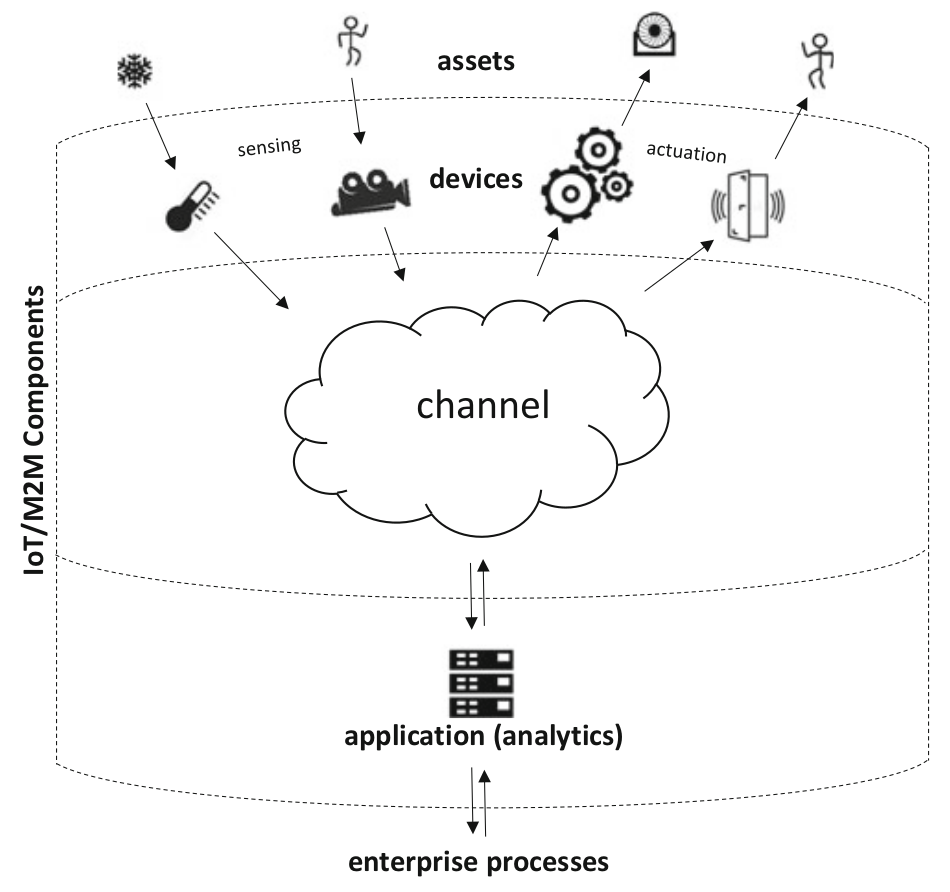
\includegraphics[width=\linewidth,height=9cm]{Pictures/IoT Components.png}}
\caption{M2M/IoT system components}
\label{fig:IoT_components}
\end{figure}

%%%%%  From MTC to IoT  %%%%%%
Most MTC systems are built and designed in a vertical way. This means that they deal with one type of parameter (e.g., position, humidity, pressure, temperature, ...) and satisfy a particular use case (e.g., turn on/off a switch). The heterogeneous nature of MTC applications leads to a wide range of proprietary networking protocols that serve a single purpose. This lack of standardization has limited the interaction between different applications and slowed the full automation transition. A horizontal expansion is required to accommodate the need for inter-operability between differen applications. Existing for many years and showing its efficiency, the Internet Protocol (IP) was the logical candidate to enable this move. An IP-based connectivity framework, that links the devices with servers running the applications, is the typical form of today's IoT systems. Figure \ref{fig:M2M_vs_IoT} illustrates the main difference between MTC and IoT systems.
\begin{figure}
\centerline{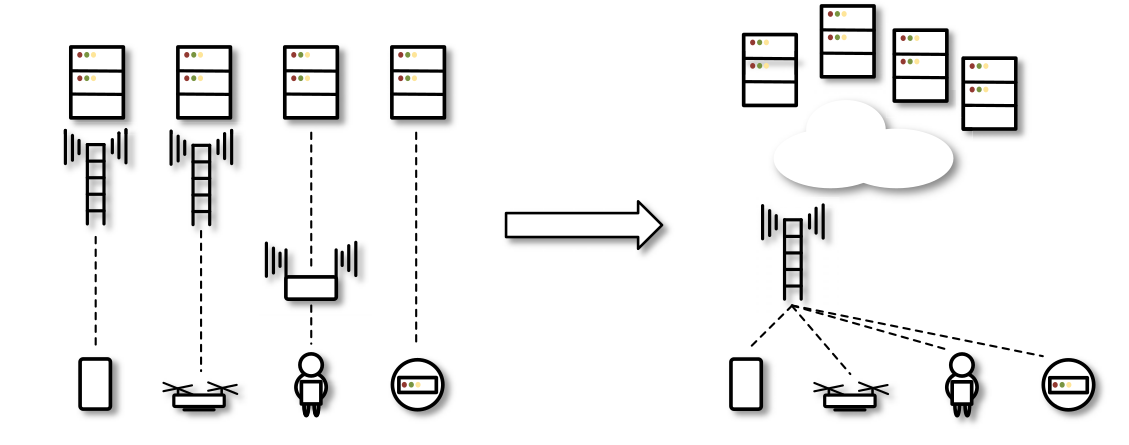
\includegraphics[width=\linewidth,height=5cm]{Pictures/M2M to IoT.png}}
\caption{M2M vs IoT Systems}
\label{fig:M2M_vs_IoT}
\end{figure}

% \begin{figure}
% \centerline{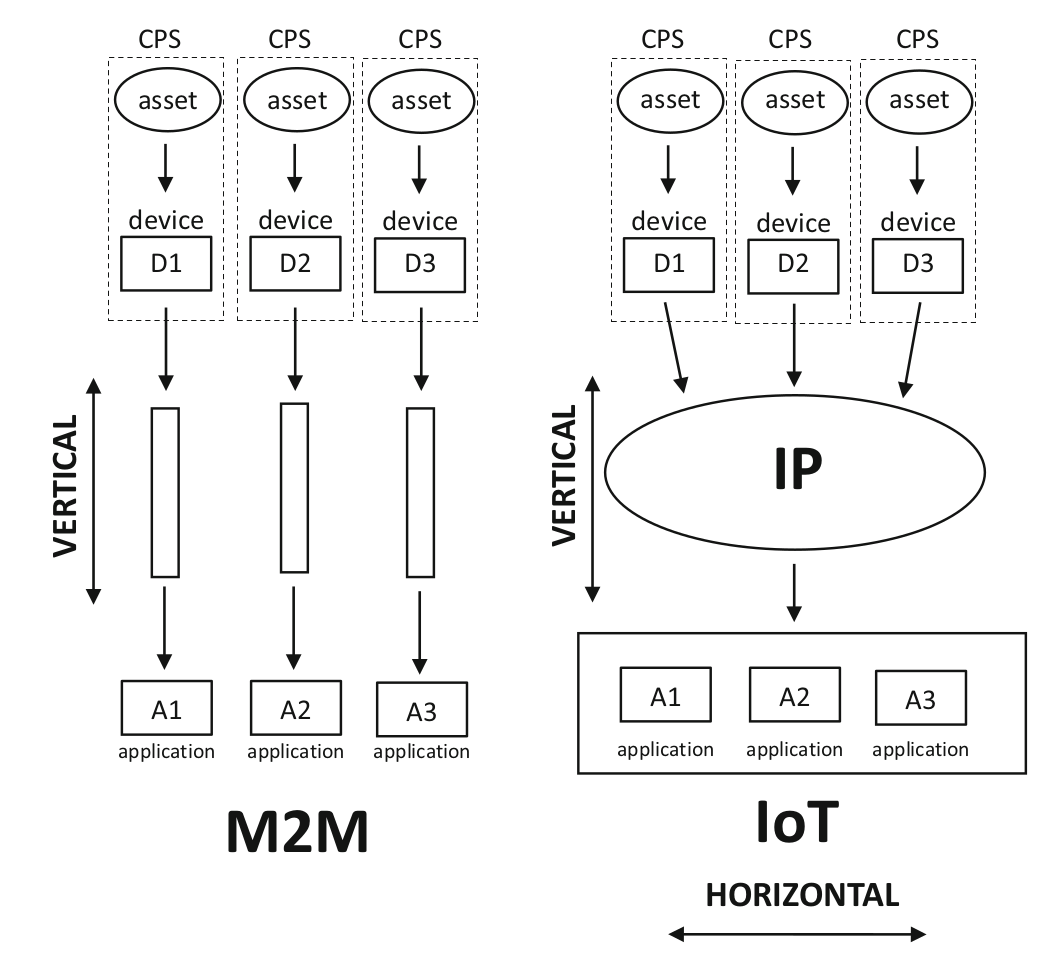
\includegraphics[width=\linewidth]{Pictures/M2M to IoT 2.png}}
% \caption{M2M vs. IoT Systems 2}
% \label{fig:M2M_vs_IoT2}
% \end{figure}

%%%%%  What is IoT  %%%%%%
No unified definition of IoT systems was agreed on worldwide, where every company adopts one aligned with its market strategy.
%     A network connecting (either wired or wireless) devices, or ‘things’, that is characterized by autonomous
% provisioning, management, and monitoring. The IoT is innately analytical and integrated (IDC)
%     IoT is the next evolution of the Internet, connecting the unconnected people, processes, data, and things in
% your business today (Cisco)
%     IoT devices as those capable of two‐way data transmission (excluding passive sensors and RFID tags). It
% includes connections using multiple communication methods such as cellular, short range and others.
% (GSMA)
%     Sensors & actuators connected by networks to computing systems. These systems can monitor or manage connected objects and machines'
% health and actions
% health and actions of connected objects and machines. Connected sensors can also monitor the natural world,
% people, and animal” (McKinsey)
However, in 2012, the International Telecommunication Union (ITU) has defined IoT systems in a more general way as follows \cite{itu-t_overview_2012_Y.2060}:
\begin{quote}
"A global infrastructure for the information society, enabling advanced services by interconnecting (physical and virtual) things based on existing and evolving interoperable information and communication technologies (ICT)."
\end{quote}
According to ITU, things can be perceived as \textit{physical} or \textit{virtual} objects with minimum communication capabilities allowing them to be identified and integrated into information networks. Physical objects are types of equipment in the real world that are usually able to collect, store, and process data (e.g., sensors, controllers, actuators, ...). On the other hand, virtual things are elements of the information world that can be stored, processed, and accessed, such as software applications and multimedia content. It's important to note that the advancement of IoT is based on the foundations of existing and evolving information and telecommunication technologies, including Artificial Intelligence (AI), big data, cloud infrastructure, and wireless networks.


%%%%%  IoT Networks: Characteristics/Requirements %%%%%%
From a networking perspective, IoT is a network of networks connected through some communications and information infrastructure. IoT networks share some defining characteristics that can differ from one use case to another. Here is a list of features that are generally associated with IoT networks \cite{itu-t_overview_2012_Y.2060,3gpp_service_nodate_22.368}:
\begin{itemize}
    \item Enormous scale: the number of connected devices in the network that need to be managed is magnitudes larger than traditional human-centered communication.
    \item Interconnectivity: In the foreseen vision of IoT, all devices must be interconnected to a global communication infrastructure.
    \item Heterogeneity: Devices in IoT are based on different hardware and connected through variable information and communication platforms.
    \item Sporadic nature: The network parameters (e.g., the number of connected devices, their location, and traffic) vary in a very dynamic and unpredictable way.
    \item Low-capability devices: In most IoT applications, devices are battery-powered and should autonomously work for several years. This imposes that IoT devices must have low processing capacity to minimize power consumption.
    \item Small infrequent data transmission: The network should be optimized to support the exchange of a small amount of data with minimum overhead.
    \item Simple design: It is essential to have a light communication protocol and network architecture to meet the limited capabilities of IoT devices.
    \item Extended Coverage: Most IoT devices are located inside buildings and have an undermined coverage due to their limitation in size and power. Therefore, providing good coverage is one of the main challenges of IoT networks.
    \item Other requirements: Some additional high-level requirements, such as identification, authentication, charging, and security, are relevant to the IoT systems. These functions can be addressed either using services provided by an intermediary network or using some proprietary solutions.
\end{itemize}

%%%%%  What is the classification of IoT applications based on requirements? %%%%%%
Based on the various presented characteristics, IoT applications can be grouped into several categories. One way of classifying IoT applications is the proposal of Ericsson which groups IoT applications into four segments that cover almost all use cases in multiple domains. These segments are Massive IoT, Broadband IoT, Critical IoT, and Industrial Automation IoT as described in \cite{kuhlins_cellular_2020} and illustrated in figure \ref{fig:IoT_applications} \cite{zaidi_cellular_2020}. a brief summary of these segments is provided in the following.

\subsubsection*{Massive IoT} describes applications where a very large number of low-capability endpoint devices sporadically transmit a small volume of data. These applications in most cases are data collection applications like sensors that read the temperature, humidity, pressure, etc. Massive IoT devices are expected to work for many years ($>10$years) without the need to replace or change their battery.

\subsubsection*{Broadband IoT} includes applications that require lower latency and higher throughput than the massive IoT. Wearables, drones, augmented reality, and virtual reality devices 
are typical examples of Broadband IoT.

\subsubsection*{Critical IoT} Unlike massive IoT, a fewer number of devices are expected to be connected to the network with relaxed constraints on the requested throughput. However, the main performance requirement needed is to guarantee a real-time reliable data transmission. One use case of this category is autonomous vehicles.

\subsubsection*{Industrial Automation IoT} This segment focuses on the integration of wireless IoT connectivity to the industrial wired infrastructure. IIoT is useful to achieve higher productivity and optimize the production process.


The different segments of IoT networks have different performance demands and only one connectivity technology can fit them all. Several types of connectivity solutions have been used to serve IoT applications including Cellular technologies and unlicensed ones. In the remainder of this article, we discuss the various IoT standards with a main focus on the newest cellular technology Reduced Capability (NR Red Cap).
\begin{figure}
\centerline{\includegraphics[width=\linewidth]{Pictures/IoT applications.png}}
\caption{IoT Networks Classifications}
\label{fig:IoT_applications}
\end{figure}




%%%%%   What the reader is expected to see in the current article?  %%%%%%
\underline{TO BE EDITED:} \emph{It is intended to provide updated information for the practitioners and help them 1) select the IoT technology 2) understand what technology will be shortly available. The goal of this article is to review, analyze and discuss recent developments observed in standardization}

\textit{(Optionally) we can add a figure showing the wide range of application and the different use cases  use supported. Like the one in by Nokia \ref{fig:iot-use-cases}.}

\begin{figure}
    \centering
    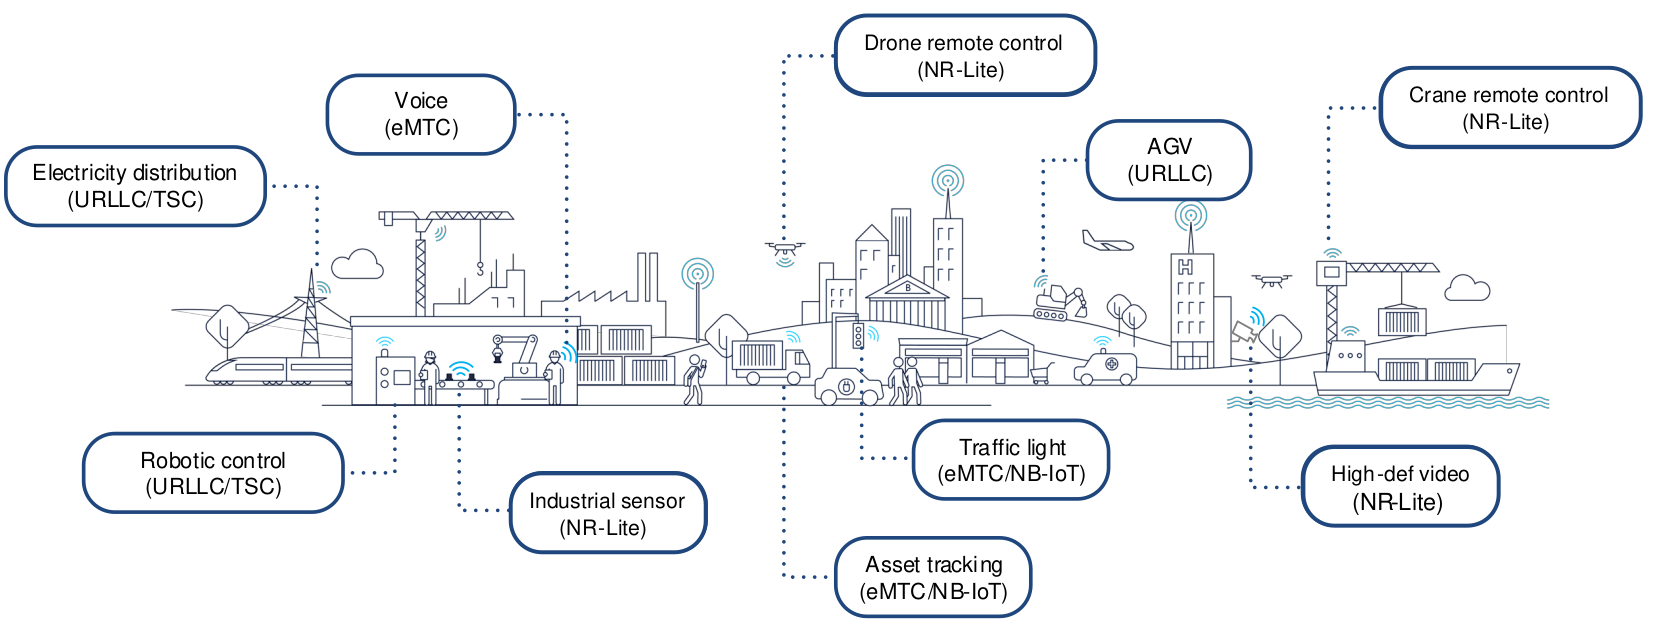
\includegraphics[width=\linewidth]{Pictures/IoT Use Cases.png}
    \caption{IoT use cases}
    \label{fig:iot-use-cases}
\end{figure}






\section{State-of-the-Art of IoT Connectivity}
\label{sec:2-IoT-Connectivity}


%   Try to Put the best reference that explains each technology and critique them

% This section tries to answer the following questions:
%     -   What are the existing IoT solutions/technologies for IoT Connectivity?
%     -   What is the current deployment in the market of each of these technologies?
%     -   What are the main features of each of them?
%     -   A preamble to the next section? (The emerge of new application and the birth of RedCap in 5G)range


%%%%%   The importance and challenges of IoT connectivity?  %%%%%%
Providing large-scale stable connectivity is considered the main challenge in order to achieve the ultimate goal of the IoT world. As presented before, IoT applications extremely vary in terms of Quality of Service (QoS) and network requirements. Such a wide diversity makes it almost impossible to have single communication technology that fits all IoT segments\cite{vaezi_cellular_2022_2}. 
%%%%%   Wired vs Wireless?  %%%%%%
Wired networks are able to provide extremely reliable connectivity with high data rates and low latency. However, the cost of installation and rigid architecture has limited their exploitation in IoT use cases. On the other hand, the re-configurable and dynamic nature of wireless communications and the recent advancement in achievable capacity and latency make them the perfect candidates for IoT connectivity.

%%%%%  ways to classify Wireless networks  %%%%%%
Wireless technologies can be classified based on the QoS they offer, i.e., coverage range (short, medium, long), data rate (high or low), latency, cost/complexity, etc. Another common way to group wireless protocols is based on the used frequency spectrum where one can find licensed and unlicensed technologies \cite{xu_narrowband_2018_3}. The choice of an adequate connectivity solution depends on several factors, such as deployment cost, coverage, and power consumption.

%%%%%  Technologies for short/medium range IoT applications  %%%%%%
Most of today's indoor IoT applications rely on short/medium-range unlicensed wireless technologies. These technologies are designed to achieve coverage of tens to hundreds of meters, which is perfect for providing the connectivity of personal and local devices.I Medium-range solutions (e.g., WiFi, Zigbee,...) are a perfect fit for home automation scenarios. Furthermore, Bluetooth and Bluetooth low-energy (BLE) are used more for fitness and medical wearables \cite{vaezi_cellular_2022_2}. Finally, Radio-Frequency IDentification (RFID), with its limited data transmission and short coverage range, is widely used in most retailers as a solution for stock monitoring and self-checkout\cite{beyene_nb-iot_2017}.


%%%%%  Technologies for short/medium range IoT applications  %%%%%%
In fact, the larger scope of IoT uses cases share common characteristics of having a large number of devices, low data rate, low power consumption, and enhanced wide coverage. Therefore, traditional short-range technologies will fail to meet the coverage requirements.  Similarly, the well-known cellular networks, namely, Global System for Mobile Communication (2G/GSM), Universal Mobile Telecommunications System (3G/UMTS), and Long Term Evolution (4G/LTE) are inappropriate for supporting most IoT applications due to their high cost, complex design, and excessive power consumption.

%%%%%  The begging of LPWA standards  %%%%%%
Given the continuing growth in the demand for IoT connectivity and the potentially enormous market, different industries have been motivated to invest and develop new revolutionary solutions that are well-suited for serving IoT communications. The main interest was developing a new Low Power Wide Area (LPWA) network class \cite{akpakwu2017survey}. Unlike conventional human-centric networks, oriented to provide high data rates and mobility, LPWA networks focus on achieving wide coverage for a large number of low-cost battery-powered nodes with relaxed requirements in terms of throughput and latency. A lot of IoT businesses were motivated to use LPWAs as a connectivity solution. This has accelerated the development and the rise of LPWA in the last decade \cite{hwang_survey_2019}. LPWA networks can now be classified into unlicensed spectrum technologies (e.g, LoRaWAN, and Sigfox) and licensed spectrum (e.g, NB-IoT, LTE-M, and EC-GSM). Figure \ref{fig:nb-iot} illustrate the trade-off between coverage and performance provided by different IoT standards. In the following, we further detail existing LPWA technologies since they are solely designed for IoT applications.

\begin{figure}
    \centering
    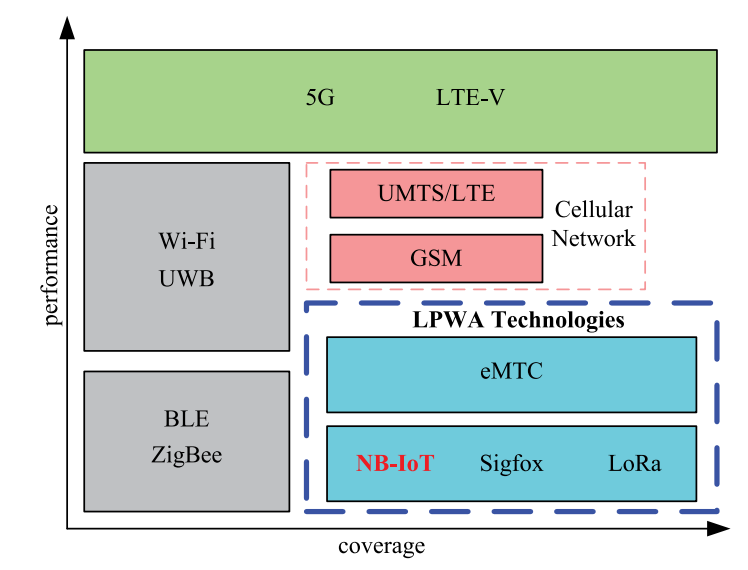
\includegraphics[width=\linewidth]{Pictures/NB-IoT example.png}
    \caption{IoT standards}
    \label{fig:nb-iot}
\end{figure}


\subsection{Standards over Unlicensed Spectrum}
\label{sec:2-1}

%%%%%  Intro to unlicensed LPWA   %%%%%%
LPWA networks over unlicensed spectrum are usually proprietary patented wireless technologies. These technologies rely on frequency resources over the industrial, scientific, and medical (ISM) bands, which will help the providers cut deployment costs. Many LPWA protocols have been developed in the last decade, including, LoRaWAN, Sigfox\cite{ayoub2018internet}, INGENU\cite{ogbodo2022survey}, TELENSA \cite{raza2017low}, and Dash7 \cite{augustin2016study}. However, the two most competitive ones that share a big part of the IoT market today are LoRaWAN and Sigfox \cite{ding_iot_2020}. More details on both of these technologies are given below.

\subsubsection{LoRaWAN}
\label{sec:2-1-1}

%%%%%  Difference between LoRa and LoRaWAN  %%%%%%
stands for Long Rang Wireless Access Network, and it is a communication protocol and system architecture developed and maintained by LoRa Alliance in 2015 \cite{LoRaWAN_spec}. \textit{LoRaWAN} is an open-source medium access control (MAC) that is based on \textit{LoRa} RF modulation technology patented for Semtech in 2014 \cite{seller_low_2016} as illustrated in Fig. \ref{fig:LoRaWAN-stack} \cite{LoRaWAN_spec}. LoRa is a proprietary spread-spectrum modulation technique that is derived from  Chirp Spread Spectrum technology (CSS) \cite{sforza_communications_2013}. CSS spreads a narrow-band signal over a wider channel bandwidth that makes the received signal more robust against interference (i.e., higher signal-to-noise-and-interference ratio (SINR)). The mathematical explanation on how LoRa modulation works is presented in \cite{vangelista2017frequency}.


\begin{figure}
    \centering
        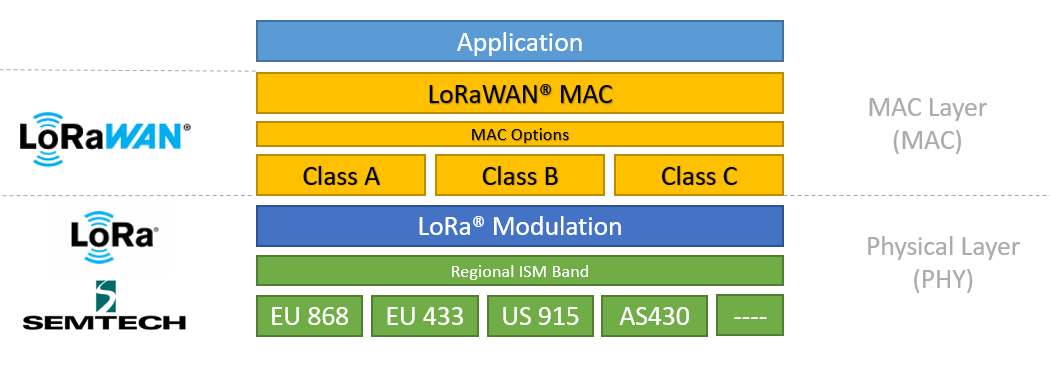
\includegraphics[width=\linewidth]{Pictures/LoRaWAN_stack-Semtech.png}
    \caption{LoRaWAN Protocol Stack}
    \label{fig:LoRaWAN-stack-Semtech}
\end{figure}

\begin{figure}
    \centering
        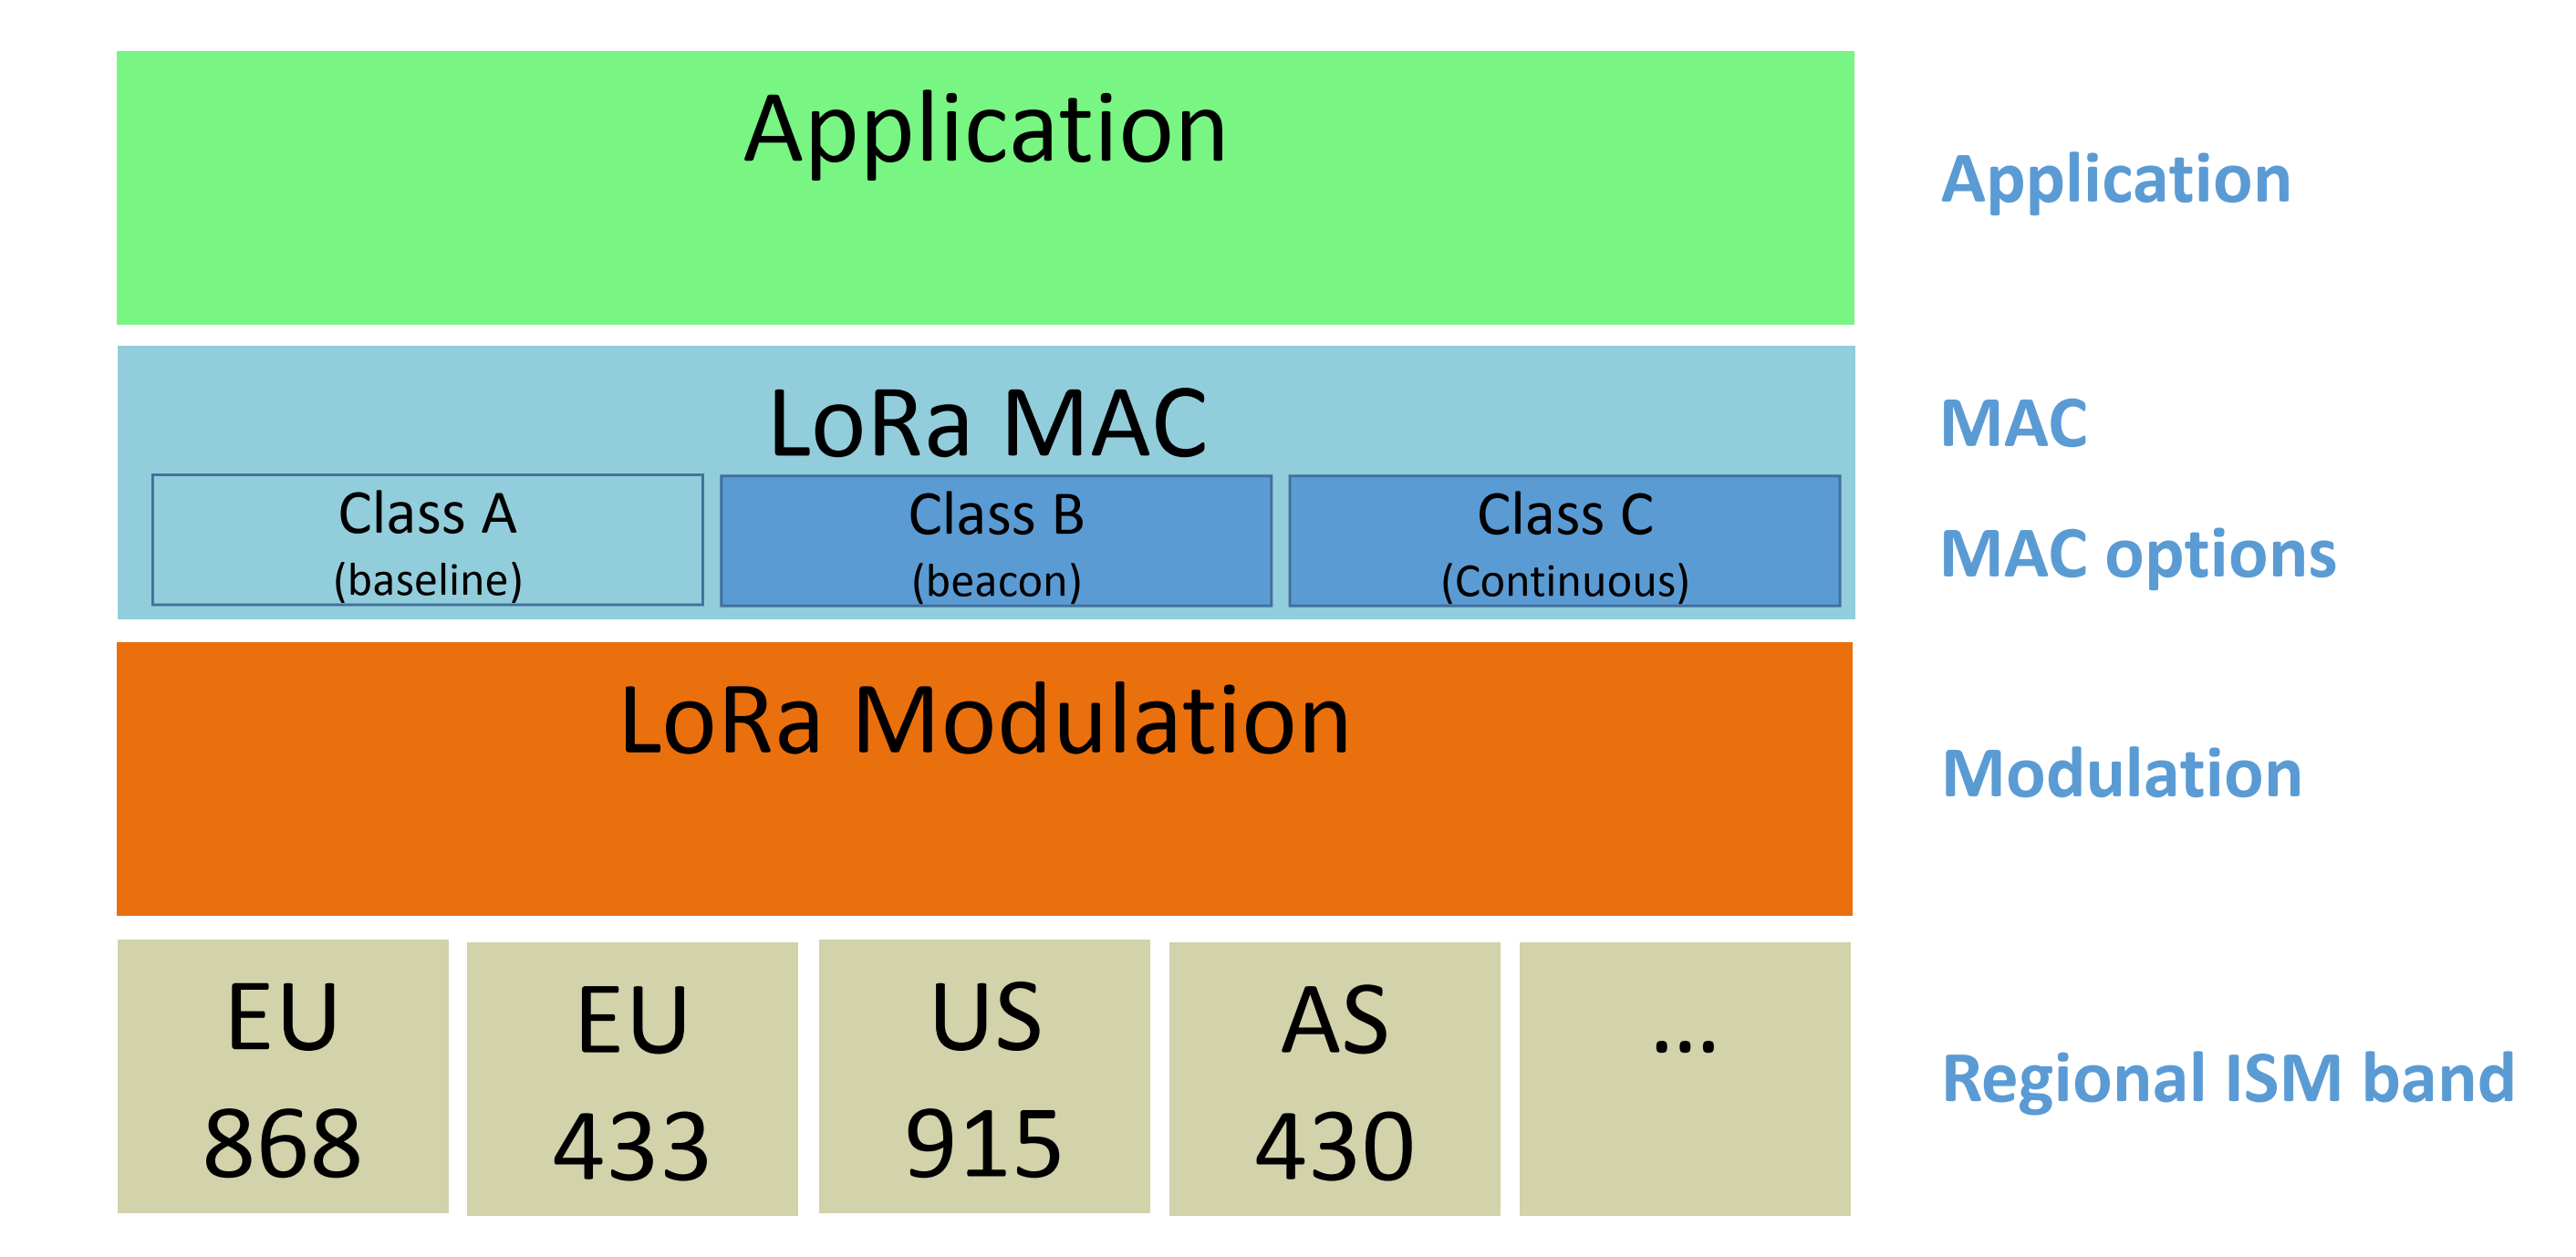
\includegraphics[width=\linewidth]{Pictures/LoRaWAN_stack.png}
    \caption{LoRaWAN Protocol Stack}
    \label{fig:LoRaWAN-stack}
\end{figure}



%%%%%  Discripe Spreading spectrum techniques  %%%%%%
Typical spreading spectrum techniques like Direct Sequence Spread Spectrum (DSSS) tend to multiply the low-rate data signal by a spreading code (so-called chip sequence) of a higher rate. This will spread the bandwidth of the original signal on a wider bandwidth corresponding to the chip rate. The spreading of the signal's bandwidth will make it more resilient to channel attenuation, like multi-path fading. This gain in the link budget is called a processing gain (Gp), and it is proportional to the $log10$ ratio of the chip rate and the data signal rate \cite{LoRaWAN_semtech}.  Spread Spectrum techniques are used in a lot of applications like military communication since it provides a more robust and secure connection.

%%%%%  Describe the LoRa modulation  %%%%%%
A similar technique is used in LoRa modulation, where the data signal is spread over a wider bandwidth using a higher rate chirp-like signal. A chirp signal is a tone that changes its instantaneous frequency over time between two frequencies, f0 and f1 \cite{haxhibeqiri2018survey}. The spreading factor (SF) is defined as the amount of spreading code applied to the original signal. The symbol rate $R$ depends on SF following the formula \cite{vangelista2017frequency}:

\begin{equation}
R=SF\times \frac{BW}{2^{SF}}
\label{equ:SF-Rate}
\end{equation}
%%%%%  SF and the tradeoff between coverage and data rate  %%%%%%
Having a high SF will reduce the achievable data rate. However, increasing SF will increase signal robustness, and that means a longer coverage range. LoRa modulation has a total of six spreading factors (SF7 to SF12). The LoRa physical layer operates in different ISM bands depending on region 433/868-MHz in Europe, 915-MHz in the US, etc. Within these bands, multiple fixed channels of  125 KHz, 200 KHz, and 500 KHz are available for UL/DL transmissions \cite{adelantado2017understanding}. Depending on the SF and channel bandwidth, LoRa data rate varies between 50kbps and 300kbps \cite{LoRaWAN_spec}. Choosing the appropriate SF is a tradeoff between data rate and coverage \cite{boisguene_survey_2017}.


%%%%%  LoRaWAN Network Elements  %%%%%%
LoRaWAN networks have three main components: End Devices, Gateways, and Network Servers. The architecture of LoRaWAN networks is organized in a star-of-stars topology where the gateways transparently relay the messages between end devices and the central network server that runs applications at the backend \cite{LoRaWAN_spec}.
%%%%%  LoRaWAN Device Classes  %%%%%%
In LoRaWAN, there are three categories of end devices with different capabilities ranging from class A, B, to C\cite{ding_iot_2020}. Class A represents end devices with the minimum functionality to work in LoRaWAN networks. Class A devices provide the lowest power consumption
and are used for applications where the communication is triggered by the end device. Downlink transmissions from the server are performed only after a received message from an end device. Class B devices are designed to allow extra downlink transmissions. End devices have a receive window at scheduled times where they should listen for incoming messages. Gateway will communicate to end devices a time-synchronized Beacon where it should be active. Finally, class C devices have nearly continuously received Windows, which reduces the latency for server-to-end-device communication \cite{LoRaWAN_spec}. Class C consumes the most power, and it is suitable for end devices that are connected to a power supply network, like traffic lights. All the devices must be compatible with Class A \cite{haxhibeqiri2018survey}. More details on the different classes of LoRaWAN and different MAC layer structures can be found in ITU-T standard Y.4480 \cite{ITU-T-Y.4480}.

\subsubsection{Sigfox}
\label{sec:2-1-2}
%%%%%  The beginiging of SigFox  %%%%%%
Another well-known LPWAs technology that runs over unlicensed spectrums is Sigfox network. Sigfox is a LPWA networking protocol that was founded by a French start-up that holds the same name in 2009 and, later, in 2022, the ownership was transferred to UnaBiz \cite{grignon_unabiz_2022}. 

%%%%%  Intro to SigFox  %%%%%%
Sigfox network can be considered as a type of cellular network, but instead of targeting human-centered applications (that require low latency and high throughput), the main goal is to serve massive IoT use cases that need ubiquitous coverage combined with lower power consumption and lower cost \cite{margelis2015low}.
%%%%%  The architecture of sigfox network  %%%%%%
The network is based on one-hop star topology where end devices are connected to gateways/base stations that convey their messages to the sigfox cloud platform backend managed by the Sigfox company itself \cite{kalfus2016ultra}. Sigfox Network Operators (SNOs) install proprietary base stations and connect them to the backend servers through an IP-based network \cite{raza2017low}. Each gateway is able to serve up to a million end-devices with a coverage of 30–50 km in rural areas and 3–10 km in urban areas \cite{augustin2016study}.

%%%%%  Explain the technology of sigfox  %%%%%%
The initial version of Sigfox was designed to support only UL communication, but later it became a bidirectional communication technology. Even though downlink transmissions are still only triggered by end devices through an uplink transmission\cite{ding_iot_2020}. The messages between base stations and end devices are modulated using Differential Binary Phase-Shift Keying (DBPSK) for UL and Gaussian Frequency-Shift Keying (GFSK) for the DL \cite{kalfus2016ultra}. Sigfox signal is carried over an ultra-narrow band (UNB) of 100 Hz in sub-GHZ ISM bands \cite{mekki2019comparative}. The main advantage of using UNB is to reduce the noise contribution on the occupied bandwidth, and therefore with the same targeted error probability; the signal can reach much longer distances \cite{do2014interference}. Each message is typically transmitted by default three times on different subchannels to increase the reliability since no acknowledgment functionality is applied \cite{margelis2015low}. In this regime and given the regulation on the emission over ISM bands, end-device can send up to 140 messages per day, with a payload size of 12 octets, at a data rate up to 100 bps \cite{augustin2016study} and using the 3-repetitions scheme the message takes around 6 s to be transmitted \cite{kalfus2016ultra}. It is worth noting that Sigfox does not provide any kind of security functionality, and it is up to the customer to adopt some technique in the application layer\cite{margelis2015low}. Sigfox is considered a complementary solution to other communication systems and can be used together with any other type of network, e.g.: Wi-Fi, Bluetooth, GPRS, NB-IoT, LoraWAN, etc \cite{noauthor_what_nodate}. The fact that Sigfox DL traffic is triggered by UL polling makes it more suitable for data acquisition applications rather than command-and-control ones \cite{augustin2016study}. No detailed specification on the standard is available for the public, but extra details are found in the patent published by sigfox in 2013 \cite{vertes2017method}.



\subsection{Standards over Licensed Spectrum}
\label{sec:2-2}

%%%%%  The problem with traditional cellular network  %%%%%%
Traditional cellular networks (i.e., 2G/3G/4G) have historically been designed to provide high-quality mobile voice and data services \cite{noauthor_how_nodate}. They have proven their ability to deal with a large amount of traffic over a wide coverage area with a better performance in terms of data rate and latency than LoRaWAN or SigFox \cite{hwang_survey_2019}. However, IoT applications cannot simply be served by existing cellular systems. Cellular systems have a limited capacity, and supporting an enormous number of terminals would be challenging, especially with the existing resource allocation approaches. For example, in LTE, for each transmission, a minimum of an entire Resource Block (RB) of 180 kHz is used \cite{accurso_exploring_2021}. This would be beneficial to reduce the signaling overhead for some applications, but for IoT traffic, it is extreme and will waste the network resources and subsequently deteriorate the overall performance. Another aspect of the problem is that IoT devices are meant to be low-end and battery-powered modules that should last for years, and supporting complex systems like cellular networks is unfeasible with such limited capabilities.
%%%%%  The problem with Unlicensed networks  %%%%%%
On the other hand, the aforementioned unlicensed spectrum technologies have some drawbacks that make them not suitable for all IoT use cases. Their lack of efficient backhaul can limit their capacity. Also, being dependent on the unlicensed spectrum will make the connection less reliable and susceptible to interference from other applications that use the same frequency \cite{hwang_survey_2019}. Therefore following the emergence of the IoT market, 3GPP since its Release 13 has started the work on developing additional IoT connectivity solutions based on existing cellular technologies to accommodate IoT growth. 

%%%%%  The beginiging of CIoT   %%%%%%
The work in 3GPP to support MTC communication over cellular networks goes back as far as Rel-8 where a technical report TR 22.868 \cite{TR_22.868} was published under the title "Study on Facilitating Machine to Machine Communication in 3GPP Systems". The early work in Rel-8 to Rel-11 was focused on the overload and congestion problem on data and signaling planes, and the shortage of resources to guarantee access for a large number of terminals \cite{benhiba_comparative_2018}. Several features were developed under the umbrella of Cellular IoT to meet the demanding IoT requirements, especially in terms of coverage enhancement, connection density, and energy efficiency. 
%%%%%  CIoT in Rel-12  %%%%%%
By the time of Rel-12, most cellular IoT deployments were relying on GSM/GPRS networks, due to their widespread coverage and low-cost UE. However, the non-optimal spectrum usage of GSM/GPRS compared to LTE has encouraged 3GPP to start the work on developing MTC UEs for LTE networks. A Study on Provision of Low-Cost MTC UEs Based on LTE was published in the technical report (TR) TR 36.888 \cite{TR_36.888}, and this was the born of LTE for MTC technology, the so-called eMTC or LTE-M now.
%%%%%  CIoT in Rel-13 %%%%%%
Later in Rel-13, a study on Extended Coverage GSM (EC-GSM) and  Narrow-Band Internet of Things (NB-IoT) technologies was initiated by 3GPP's technical specification group GSM EGPRS RAN (GERAN) \cite{liberg_cellular_2019}. This study aimed to investigate the feasibility of supporting ultra-low complexity and low-throughput IoT applications over cellular systems. The findings of this study were later documented in TR 45.820 \cite{TR_45.820}.
%%%%%  CIoT after Rel-13 %%%%%%
After Rel-13 TSG GERAN was closed and its responsibilities were transferred to TSG RAN took charge of developing both EC-GSM and NB-IoT along with LTE-M \cite{liberg_cellular_2019}. These technologies are the representatives of LPWA standards operating on the licensed spectrum \cite{adelantado2017understanding}, and they are widely deployed around the world \cite{noauthor_mobile_nodate}. A more detailed comparison between Cellular IoT technologies is presented in the following.

\subsubsection{LTE-M}
\label{sec:2-2-2}
%%%%%  Define LTE-M %%%%%%
is a cellular IoT standard based on the legacy LTE network. LTE-M is considered a simplified version of 4G networks optimized to support scenarios that require medium to low rates, wide coverage, a high number of connections, and extended battery lifetime\cite{benhiba_comparative_2018}.
%%%%%  the beginning LTE-M %%%%%%
In Rel-12, 3GPP initiated the work of LTE-M by introducing a new category of MTC devices (so-called, Cat-0) as low-cost MTC devices \cite{rico2016overview}. LTE-M devices use typical 4G multiple access techniques of orthogonal frequency division multiple access (OFDMA) in the downlink and single carrier (SC-FDMA) in the uplink and share the same spectrum resources as other LTE UEs\cite{ding_iot_2020}. However, compared to its counterpart Cat-1, the lowest LTE UE category in Rel-11, Cat-0 can provide a $50\%$ of complexity/cost reduction\cite{sharma2019toward}. This gain comes from the fact that Cat-0 devices are equipped with a single RF chain (i.e., no MIMO support) and can optionally operate in Half-Duplex mode \cite{liberg_cellular_2019}. The cut in the device capabilities will limit UL/DL throughput to 1 Mbps \cite{wang_information_2021}. In addition to cost gain, LTE-M devices will enjoy a longer battery lifetime ($\sim$10 years \cite{GSM_white_2018}) due to the newly introduced UE power-saving techniques, namely, extended Discontinuous Reception (eDRx) and Power Saving Mode (PSM)\cite{raza2017low}.
%%%%%  Enhanced features of LTE-M %%%%%%
In Rel-13, 3GPP launched a new category of LTE-M devices, known as enhanced MTC (eMTC), or equivalently (Cat-M/Cat-M1). This category aims to further reduce device capabilities and cater to lower IoT applications. Cat-M devices have a restricted bandwidth of 1.4 MHz instead of 20 MHz, but an extended coverage (15 dB more than the conventional LTE coverage\cite{xu_narrowband_2018_3}) using more repetition in the time domain. Devices of this class are 25 $\%$  cheaper than original Cat-0 LTE-M devices and still provide relatively the same throughput of 1 Mbps\cite{herrero_fundamentals_2021}. It is worth noting that, even with their limited capabilities, Cat-M devices are able to support real-time functionalities like voice over LTE (VoLTE)\cite{foubert2020long}.
%%%%%  LTE-M deployment %%%%%%
The deployment of LTE-M network is spread all over the world \cite{foubert2020long}. Many MNOs were able to support LTE-M devices using their legacy LTE network. LTE-M operates over the same spectrum resources as LTE and only a software update to the network is required to support it without any physical hardware modification \cite{chaudhari2020lpwan}.






\subsubsection{Narrow-Band IoT (NB-IoT)}
\label{sec:2-2-1}
NB-IoT is a narrow-band cellular LPWAN technology that was standardized by 3GPP in Rel-13 in 2016\cite{TR_45.820}. It aims to provide wider coverage, lower device cost, longer battery life, and higher connection density compared to LTE-M \cite{ding_iot_2020}. NB-IoT is another deviation of LTE and is based on its functionalities and network architecture. NB-IoT was introduced as a new category of MTC devices, so-called Cat-NB1/Cat-NB2 \cite{liberg_cellular_2019}. It can coexist with GSM and LTE in sub-GHz deployments \cite{chaudhari2020lpwan}, where three modes of operations are adopted \cite{chen2017narrow,chettri_comprehensive_2020_1}:
 \begin{itemize}
     \item Independent (stand-alone) operation: It is based on utilizing and re-framing any available spectrum of GSM carriers in the form of 200 KHz channels.
     \item Guard-band operation: this mode makes use of the available resource blocks in the unexploited guard band of LTE carrier frequency.
     \item In-band operation: it utilizes the same frequency resource blocks available within LTE carriers. 
 \end{itemize}
An illustration of NB-IoT deployment modes is shown in Fig. \ref{fig:NB-IoT-deployments}. Deploying NB-IoT in sub-GHz bands (i.e., 700MHz, 800MHz, and 900MHz licensed frequencies) makes it an excellent choice for providing extensive coverage. 
\begin{figure}
    \centering
        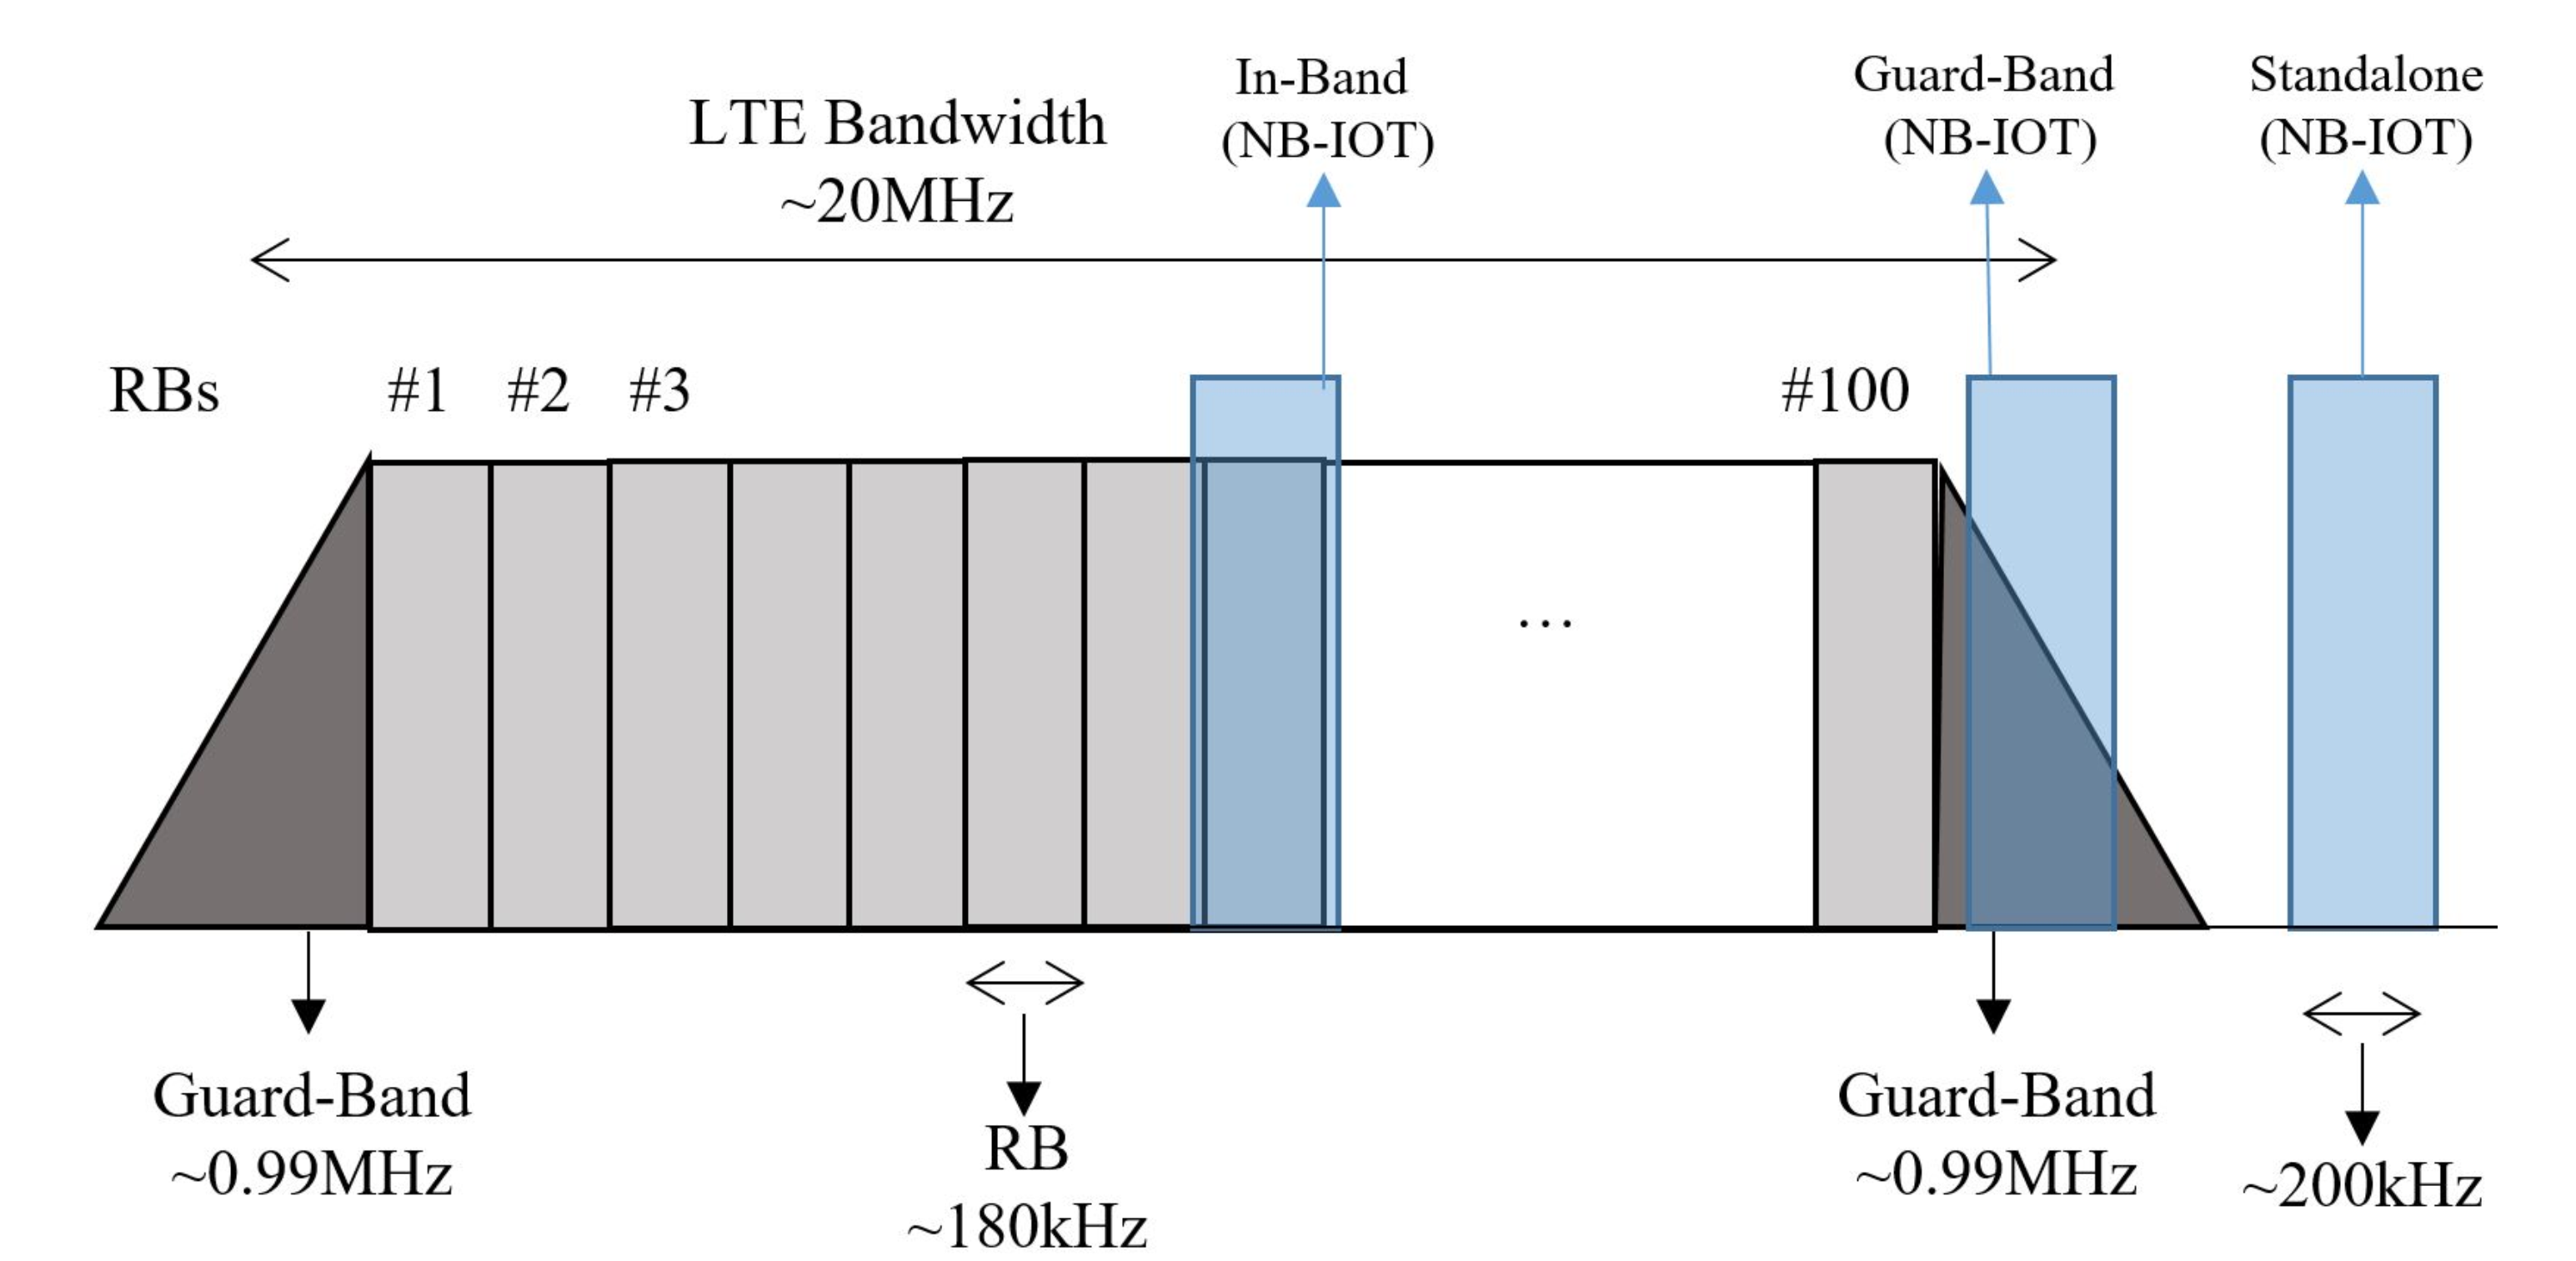
\includegraphics[width=\linewidth]{Pictures/Deployments supported by NB-IoT.png}
    \caption{Deployment modes for NB-IoT}
    \label{fig:NB-IoT-deployments}
\end{figure}
The NB-IoT network is able to support a link budget of 164dB which is 20 dB stronger than the traditional GSM and LTE network\cite{hwang_survey_2019} while serving up to 50,000 UEs per cell with the possibility to scale up the capacity by allocating more carriers for NB-IoT\cite{raza2017low}. It is worth noting that, independent and guard-band modes are able to provide better indoor coverage since the received signal will not suffer from the same interference experienced in the In-band mode \cite{poursafar2017long}.
NB-IoT supports bi-directional communication using OFDM for the downlink and SC-FDMA for the uplink, and unlike LTE-M only half-duplex operations are supported \cite{ding_iot_2020}. The NB-IoT small bandwidth of NB-IoT (only 180 kHz) helps cut the cost and energy consumption at the expense of reducing the data rate ($> 50$ kHz\cite{rico2016overview}) and increasing the latency. In addition, even though NB-IoT was built on top of the legacy LTE network, it can be considered as a new interface from the protocol stack point of view\cite{mekki2019comparative}. Many optimizations have been adopted to both the control plane and user plane in order to support the transmission of small data packets \cite{sharma2019toward} (e.g., multiple transmissions are carried on one RB \cite{accurso_exploring_2021}). A simplified mobility function is provided with no handover support technology \cite{foubert2020long}, and due to the narrow bandwidth of NB-IoT, new physical channels were introduced for synchronization, cell search, as well as new reference signals for channel estimation, tracking, and demodulation\cite{rico2016overview}. Regarding UE power-saving, the same techniques of PSM and eDRX are re-used in NB-IoT with more extended sleeping periods\cite{vaezi_cellular_2022_2}.  More detailed information on NB-IoT specifications and features we refer to the following resources \cite{wang2017primer,chen2017narrow} 



\subsubsection{EC-GSM}
\label{sec:2-2-3}
is standard-based technology developed by 3GPP as one of the promising candidates for LPWA CIoT. The work on EC-GSM started in 2015 as part of Rel-13 \cite{TR_45.820} along with NB-IoT. It is based on eGPRS technology and can be deployed to existing GSM networks through a software upgrade \cite{poursafar2017long}. The traffic of legacy GSM devices and EC-GSM-IoT is multiplexed on the same physical channels \cite{chaudhari2020lpwan} and operates over the GSM 850–900 and 1800–1900 MHz bands \cite{herrero_fundamentals_2021}. EC-GSM channels have a bandwidth of 200 kHz, whereas conventional tools of combining FDMA with TDMA are used for multiple access \cite{liberg_cellular_2019}. 
Two modulation techniques are used, namely Gaussian Minimum Shift Keying (GMSK) and 8PSK, providing a peak data rate of 70 and 240 kbps, respectively \cite{raza2017low}. It offers an improvement of 20 dB in the coverage compared to the typical GSM coverage\cite{hwang_survey_2019} allowing the signal to reach locations with challenging conditions such as deep indoor basements \cite{chaudhari2020lpwan}. EC-GSM is also designed to support low-complexity and low-energy devices with a battery life of up to 10 years \cite{poursafar2017long}.
Even though this GSM-based technology provides a performance equivalent to NB-IoT, and can be extremely useful for supporting low-end IoT applications, it does not get the same attention as its two counterparts CIoTs \cite{foubert2020long}. This is because a lot of mobile operators are planning to shut down their 2G/3G deployments in order to free up some resources for the upcoming 5G network \cite{noauthor_complete_2019}.






Table \ref{table:LPWA-technologies} summarize the different features of the main LPWA technologies presented in this section. It can be seen rom Table \ref{table:LPWA-technologies} that all LPWAN technologies (Licensed and Unlicensed) support a wide-area coverage with a long battery lifetime at the expense of a low data rate.


\begin{table*}
\centering
\caption{Comparison of different LPWA technologies }
\begin{tabular}{|c | c | c | c| c| c|} 
 \hline
  \multirow{2}{*} {\textbf{Feature}} & \multicolumn{2}{c|}{\textbf{non-3GPP}}  &  \multicolumn{3}{c|}{\textbf{3GPP}} \\
  \cline {2-6}  
    & \textbf{LoRaWAN} & \textbf{Sigfox} & \textbf{NB-IoT} & \textbf{LTE-M} & \textbf{EC-GSM} \\ 
\hline
 Random access & ALOHA/Slotted-ALOHA & ALOHA & NPRACH & PRACH & RACH\\
 \hline
  Modulation type & CSS & GFSK/DBPSK & BPSK/QPSK & QPSK/QAM & GMSK/8PSK\\
 \hline
  Devices per cell & 10K & 10K & 50K & 18K & 20K\\
  
 \hline
  Maximum Coupling Loss & 157 dB & 153 dB & 164 dB & 154 dB & 164 dB\\

   \hline
  Coverage Range & $<15 km$ & $<50 km$ & $<15 km$ & $<11 km$ & $<15 km$\\
 \hline
 
  Duplex Mode  & Half-duplex & Half-duplex & Half-duplex & Full/Half-Duplex & Half-Duplex\\

 \hline

\multirow{2}{*} {Channel Bandwidth} & \multirow{2}{*} {125-500 kHz} & \multirow{2}{*} {100 Hz} & 180 kHz(LTE carrier) & 20 MHz (LTE Cat-0) & \multirow{2}{*} {200 kHz} \\ 
& & &200 kHz(GSM carrier) & 1.4 MHz (LTE Cat-M1) & \\

  \hline  
  
  MAC Solution & Spread Spectrum &   UNB    & OFDM/SC-FDMA &  OFDM/SC-FDMA &  TDMA/FDMA \\

  \hline
  
  Peak Rate & 50-300 kbps & 100 bps & 250 kbps & 1 Mbps & 70-240 kbps   \\
  
 \hline
 
 Voice Support  &   No  &   No  &   No  &   Yes (VoLTE)  &   No  \\
 
 \hline
 
  Mobility Support & Yes & No & Limited & Yes & Limited\\

  
    \hline
  
  Module Cost\cite{foubert2020long} &  $9–12$ dollars &  $5–10$ dollars&  $7–12$ dollars& $10–15$ dollars &  $\$\sim5$ dollars   \\
  
 \hline
 
   Battery lifetime & \multicolumn{5}{c|}{$> 10$ years}\\
  
  \hline
  Localization Support& \multicolumn{5}{c|}{Yes}\\
  
  \hline
\end{tabular}
\label{table:LPWA-technologies}
\end{table*}


\section{Reduced Capability Devices}
\label{sec:3-RedCap-Intro}

% This section tries to answer the following questions:
%     -     What is the current state of 5G? (Existing usage scenarios)
%     -     What are the new market sectors in IoT available for 5G?
%     -     Why we need a new category to support these new use-cases? (Justification of RedCap)
%     -   What is the definition of RedCap?
%     -   What are the requirements of RedCap devices?
%     -   What is the standardization process?
%     -   Preamble to the next section?


%%%%%   The Main classes of 5G before Rel-17  %%%%%% Good
The early 5G system in Rel-15 was originally intended to support three main usage scenarios, namely, enhanced mobile broadband (eMBB), ultra-reliable and low-latency communications (URLLC), and massive machine type communications (mMTC). These three classes have significantly heterogeneous requirements in terms of data rate, latency, connection density, energy efficiency, reliability, and mobility. ITU has identified the minimum technical performance requirements for 5G services known as the IMT-2020 standard. These features have been summarized in the report M.2410-0 \cite{itu-r_minimum_2017_M.2410-0}.

%%%%%   URLLC and mMTC  %%%%%%
 Both URLLC and mMTC are intended to target IoT applications. URLLC which was primarily introduced in Rel-15 addresses time-sensitive applications such as industrial operations and remote surgery. A further enhanced version of URLLC was introduced in Rel-16 within the enhanced URLLC (eURLLC) work item \cite{3gpp_study_nodate_38.824}. On the other hand, mMTC is meant to serve low-end IoT applications that have relaxed requirements in terms of data rate and latency.

%%%%%   Smart factory and vertical industries  %%%%%%
One of the important goals of 5G systems is to enable the automotive industry. The framework of Industry 4.0 aims to create more interconnected smart factories. This industrial transformation can help improve efficiency, reduce operational costs, increase safety, and enhance productivity. It is important to note that developing a massive industrial wireless sensor network is the base to achieve this foreseen transformation.

%%%%%   Smart cities  %%%%%%
Alongside smart factories, the future information society contains an important element so-called smart cities. Smart cities include the optimization of a variety of city activities such as lighting, transport, waste management, parking, video surveillance, etc. The collected data from all these applications can be used to efficiently manage and control city resources and improve provided services to residents. 5G is considered a vital enabler in this envisioned shift toward smart cities.

%%%%%   Wearables  %%%%%%
Another use case that will play an important role in the future 5G community is Wearables. Devices like smartwatches, extended reality (XR) devices, and medical devices will have a huge impact on everybody's life. The spread of 5G network will provide the connectivity needed for these new applications.

%%%%%   New mid-IoT fall in Between %%%%%%
The forenamed mid-range use cases have requirements that fall in between those of eMBB, URLLC, and mMTC. They are demanding a performance higher than what is offered by mMTC but lower than URLLC and eMBB as shown in figure \ref{fig:redcap-spider}. One can see that existing 5G usage scenarios either fail to meet the minimum requirements of mid-range IoT applications or they are too powerful which can lead to waste network resources.

\begin{figure}
    \centering
    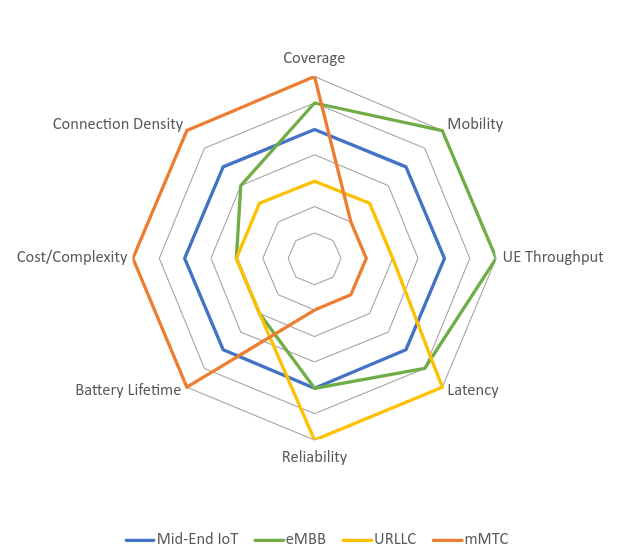
\includegraphics[width=\linewidth]{Pictures/Radar Chart RedCap.png}    
    \caption{RedCap Radar chart}
    \label{fig:redcap-spider}
\end{figure}

%%%%%   The need for new class in 5G  %%%%%%
Therefore it is important to further optimize the network and more efficiently support such mid-range IoT applications. In this regard, 3GPP has initiated in Rel-17 the work to support a new category of devices with a reduced cost/complexity compared to the high-end Rel-16 eMBB and URLLC NR devices. This new category was presented as a lightweight version of NR devices under the name of NR-Light or NR-lite. However, now it is officially called Reduced Capability devices (RedCap).

%%%%%   The introduction of RedCap  %%%%%%
The main objective of RedCap UE category is to serve three reference use cases: Industrial wireless sensors (e.g., various kinds of sensors and actuators), Video Surveillance (e.g., surveillance cameras that are essential for smart city), Wearables (e.g., AR/VR devices, Human-assistive devices, smart watches, glasses,  etc.).

%%%%%   The requirements of RedCap  %%%%%%
Table \ref{table:redcap-requirements} presents the main requirements specified by 3GPP in the study item on support of reduced capability NR devices TR 38.875 \cite{3gpp_study_2021_38.875}. From table \ref{table:redcap-requirements} it is noted that these three representative use cases have slightly different requirements. However, they can be categorized into one class of mid-end IoT services to avoid market fragmentation \cite{3gpp_framework_2020_R2-2009618}. RedCap devices share common generic constraints of being low cost/complexity and compact in size. They are also meant to support 5G frequency bands in both frequency range 1 (FR1), and frequency range 2 (FR2), and support the two modes of operation: frequency division duplex (FDD) and time division duplex (TDD).

\begin{table*}
\centering
\caption{Redcap reference use cases and requirements}
\begin{tabular}{|c | c | c | c|} 
 \hline
 \textbf{Requirement} & \textbf{Industrial wireless sensors} & \textbf{Video Surveillance} & \textbf{Wearables} \\ 
 \hline
 Data Rate & \multirow{2}{*} {2 Mbps} & \multirow{2}{*} {7.5-25 Mbps} & 5-50 Mbps in DL (peak 150 Mbps)\\ 
  & & & 2-5 Mbps in UL (peak 50 Mbps) \\
  \hline
 Latency & 100 ms (5-10 ms in safety applications) & 500 ms & - \\
  \hline
 Availability & $99.99\%$ & $99\%-99.9\%$ & - \\
  \hline
 Battery lifetime & few years & - &  Multiple days (up to 1-2 weeks) \\
  \hline
 Traffic pattern & Heavy UL & High-end video (Heavy UL) & - \\ 
 \hline
 Mobility & Stationary & Stationary & Low-Mobility \\
  \hline
Coverage & \multicolumn{3}{c|}{$MCL=143dB$}\\
 \hline
 Cost/Complexity & \multicolumn{3}{c|}{Low cost/complexity devices compared to eMBB and URLLC}\\
 \hline
 Size & \multicolumn{3}{c|}{a design with compact form factor}\\
 \hline
\end{tabular}
\label{table:redcap-requirements}
\end{table*}

%%%%%   Seprate RedCap from other 3GPP   %%%%%%
It is worth saying that RedCap devices approximately provide a performance similar to low-end LTE UEs such as Cat-1. Nevertheless, it was agreed to develop RedCap as a 5G standalone technology to benefit from the efficiency of the 5G core network and facilitate the transition to a full 5G society. Also, it is important to note that RedCap is not designed to serve low-power wide-area (LPWA) use cases. 3GPP confirmed in its study on "self-evaluation towards IMT-2020 submission" \cite{3gpp_study_nodate-1_37.910} that together LTE-M and NB-IoT fulfill IMT-2020 requirements for mMTC class and they will be considered as 3GPP technologies for LPWA application. Therefore RedCap design reuses NR features in the best way suited for its use cases.

%%%%%   Standardization process and preamble for next sub-section   %%%%%%
In Rel-17 The study phase on the support of RedCap devices was initiated by multiple RAN work groups. The study aimed to find technical solutions to support the new category while having a minimal impact on existing network scenarios. Three main objectives were announced for this work item: UE complexity Reduction, UE battery lifetime enhancement, and coexistence with other technologies. The following sections explain in detail the proposed features and their impact on the performance. The collected findings during the study phase are documented in the technical report TR 38.875 \cite{3gpp_study_2021_38.875}. The study phase was followed by standardization work to specify the required updates of NR standard, specifically,  UE capabilities in TS 38.306 \cite{3gpp_nr_nodate-4_38.306} and RRC parameters in TS 38.331 \cite{3gpp_nr_nodate-3_38.331} (see section 4.2.21).

\section{UE complexity reduction}
\label{sec:4-complexity-reduction}

% Note: Add more details on how the gain in cost is calculated (Small paragraph saying that each part of the device hardware has a certain gain and the overall gain is an accumulation)



% This section tries to answer the following questions:
%       -   What are the proposed features/enhancements in Rel-17 to reduce the complexity in RedCap devices?
%       -   For each of these features, we highlight:
%           -   Description
%           -   Gain in terms of cost/complexity
%           -   Potential impact on network performance


%%%%%   Emphasize that RedCap is an extension of NR UE   %%%%%%
The design of low-cost/complex devices was the main priority of the RedCap work item. RedCap devices are built on the foundation of reference Rel-15/16 NR devices. This means that RedCap will try to optimize NR configurations in a way that suits the use cases of mid-end IoT applications.

%%%%%   preamble to next subsections   %%%%%%
Many technical solutions have been suggested to reduce UE cost/complexity. Most of these modifications are related to features in the physical layer (e.g., Bandwidth, no. of antennas, etc). In the following, we present the main complexity reduction features discussed in RedCap Rel-17 \cite{3gpp_study_2021_38.875}.






\subsection{Reduced the number of UE Rx antennas}
\label{sec:4-1}

%%%%%   Feature description   %%%%%%
The support of multi-input multi-output communication is essential for most modern-day wireless systems. Increasing the number of receiving antennas (Rx), based on the applied signal processing, may dramatically enhance the experienced coverage and throughput at the user terminal. However, these desired advantages come at the cost of unpleasant complex RF chains and overhead processing. The reference NR device supports the following minimum antenna configuration:
\begin{itemize}
    \item In FR1: 2 Rx for FDD mode and 4 Rx for TDD mode
    \item In FR2: 2 Rx
\end{itemize}
While for RedCap UEs only 1 Rx, and optionally 2 Rx, was considered as the minimum requirement in the study.

%%%%%   The improvement   %%%%%%
Reducing the number of Rx branches simplifies both UE RF components (including Antenna array, Filters, LNAs, mixer, and local oscillator) and Base-Band operations (ADC/DAC, FFT/IFFT, Synchronization/cell search block, MIMO processing). The overall device cost/complexity reduction can reach $30-50\%$. More information about the evaluation methodology and the estimation of cost reduction can be found here R1-2009293 \cite{3gpp.R1-2009293}
%%%%%   Negative possible impact   %%%%%%
This cut in the device cost/complexity comes at the expense of degrading network performance. Having one Rx branch limits RedCap devices from performing MIMO operations and benefiting from spatial diversity. This may impact both coverage and spectral efficiency. Nevertheless, RedCap's requirements are still met. Another aspect concerning energy consumption, where in theory it should be reduced due to the usage of fewer Rx branches. However, the time needed to receive a certain payload is increased as a result of the degradation in the device data rate.

\subsection{UE bandwidth Reduction}
\label{sec:4-2}

%%%%%   Feature description in legacy NR   %%%%%%
Legacy NR devices must support two ranges of carrier frequencies, namely, FR1 and FR1. Within these two possible ranges, UE will transmit/receive signals over a carrier bandwidth. In 5G NR, The maximum allowed carrier bandwidth is 100 MHz in FR1 and 200 MHz (optionally 400 MHz) in FR2 (see \cite{3gpp_nr_nodate-2_38.101-1,3gpp_nr_2022-7_38.101-2}). Higher carrier bandwidth can be reached using Carrier Aggregation (CA).
%%%%%   What is done in RedCap   %%%%%%
Given the less demanding requirement of RedCap use cases in terms of data rate, it is possible to decrease the maximum supported bandwidth. For RedCap UEs, the maximum allowed bandwidth is 20 MHz in FR1 and 50 MHz (optionally 100 MHz) in FR2. It was also suggested to abandon the support of CA for RedCap device.

%%%%%   The gain   %%%%%%
This reduction in UE bandwidth results in a substantial decrease in device cost/complexity, estimated to be on the order of $\sim30\%$ in FR1 and $\sim20\%$ in  FR2. Most of the reported gain is associated with less processing in base-band parts (ADC/DAC, LDPC decoding, ...).
%%%%%   Negative possible impact   %%%%%%
It must be noted that this cut has a minor impact on coverage, spectral efficiency, and latency. The main affected metric is the achievable peak data rate. However, it is still enough to meet the predefined requirements of RedCap use cases.


\subsection{Half-duplex FDD Operation}
\label{sec:4-3}
%%%%%   Feature description in legacy NR   %%%%%%
One of the main capabilities of 5G UE is the support of duplex communication, i.e., communicate in both directions uplink and downlink. Two duplexing approaches exist: Frequency Division Duplex (FDD), and Time Division Duplex (TDD) as illustrated in figure \ref{fig:5g-duplexing}. FDD implies that UL and DL transmission occurs on different carrier frequencies. On the other hand, in TDD, the separation between the two flows takes place in the time domain. 
While FDD offers better coverage due to frequency separation, TDD provides higher throughput because of the simplified processing. In general, a reference 5G device supports both TDD and FDD modes.

 \begin{figure}
    \centering
    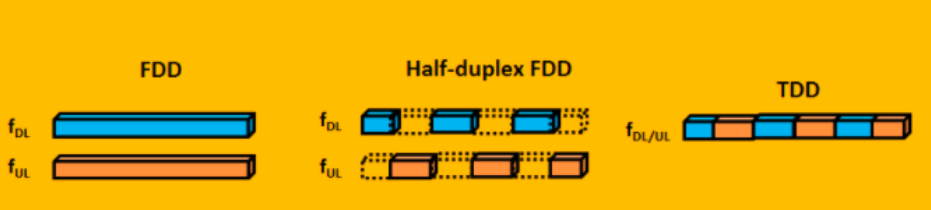
\includegraphics[width=\linewidth]{Pictures/5G Duplexing.png}
    \caption{5G Duplexing}
    \label{fig:5g-duplexing}
\end{figure}

Furthermore, FDD is divided into Full-Duplex (FD-FDD) and Half-Duplex (HD-FDD) modes. 
Full-Duplex FDD means that the transmission on both DL and UL happens at the same time. On the contrary, HD-FDD operation obligates that UE is only allowed to receive or transmit at a given time. This approach of communication gained a lot of attention in LTE for use cases that do not require high throughput but have some constrain on energy consumption such as IoT applications. In TS 36.211 \cite{3gpp_evolved_nodate_36.211}, two types of HD-FDD were defined: Type A and Type B. The main difference between the two types is the guard period between receiving and transmitting, where Type B allows a wider guard.
%%%%%   What is done in RedCap   %%%%%%
In the study phase of RedCap \cite{3gpp_study_2021_38.875}, it was suggested to use both types of HD-FDD types, where Type A is prioritized.

%%%%%   The gain   %%%%%%
Compared to a reference NR device, a RedCap device with HD-FDD system can save $\sim7\%$ for Type A and $\sim10\%$ for Type B. Most of the cost saving comes from replacing the duplexer with a switch and a low-pass filter and having a simplified RF transceiver.
%%%%%   Negative possible impact   %%%%%%
However, operating in half-duplex mode may have a negative impact on the latency. Some additional delay can be experienced especially in case of simultaneous DL and UL traffic. Nevertheless, the latency requirement for RedCap use cases is still fulfilled. Also, it is worth noting that introducing HD-FDD operation will have some impacts on the specification, e.g., determining UL/DL switching time, applicable bands, etc \cite{ratasuk_reduced_2021}. 


\subsection{Relaxed maximum number of MIMO layers}
\label{sec:4-4}

%%%%%   Feature description in legacy NR   %%%%%%
One way of using multiple antennas in wireless systems is spatial multiplexing. Spatial multiplexing is based on dividing the transmitted data into several traffic flows, so-called MIMO layers, and sending them simultaneously on different available antennas. This very powerful technique helps enhance the system's spectral efficiency and multiply the achievable data rate.
The reference NR device can support, depending on antenna configuration, up to 4 MIMO layers in FR1 and 2 layers in FR2.
%%%%%   What is done in RedCap   %%%%%%
For RedCap the maximum number of MIMO layers was reduced to one layer FR1/FR2 and optionally 2 layers for FR1 TDD.

%%%%%   The gain   %%%%%%
Reducing the maximum number of MIMO layers helps in simplifying the signal processing and eventually the overall cost/complexity. The gain in cost is $\sim17\%$ when reducing from 4 to 1 layer in FR1 TDD and $\sim11\%$ when reducing to 1 layer for the case of FR2.
%%%%%   Negative possible impact   %%%%%%
The main impact of cutting the number of supported MIMO layers is decreasing the spectral efficiency and subsequently the achievable data rate. The peak rate may decrease by $50-75\%$. Despite this reduction, RedCap devices can still be able to fulfill the defined requirements.

\subsection{Relaxed maximum modulation order}
\label{sec:4-5}

%%%%%   Feature description in legacy NR   %%%%%%
Modulation order is an important factor that affects the experienced throughput. Having a higher modulation order can dramatically increase the spectral efficiency (e.g., 256QAM=8 bits per symbol).

%%%%%   What is done in RedCap   %%%%%%
In the RedCap study and in order to cut the device cost, it was suggested to change the maximum mandatory modulation orders as follows: 64QAM instead of 256QAM for DL  and 16QAM instead of 64QAM for UL.

%%%%%   The gain   %%%%%%
The proposed relaxation of modulation orders decreases UE's cost/complexity by reducing the required processing in both RF and base-band. The estimated reduction in the cost is $\sim6\%$ for the downlink case and $\sim2\%$ for the uplink.

%%%%%   Negative possible impact   %%%%%%
Similar to the reduction of maximum MIMO layers the main impacted performance indicator here is the spectral efficiency. The peak rate will decrease by $25-33\%$, depending on the considered relaxation. Even with this degradation in the achievable throughput, the predefined requirements RedCap device are met.  

\subsection{Combinations of UE complexity reduction features}
\label{sec:4-6}
Alongside studying individual techniques listed in subsections A-E, it was suggested to mix some of them together. Different combinations of complexity reduction features and their impact on the device's overall material cost are presented in TR 38.875 (See Table 7.8.2-1, Table 7.8.2-2, and Table 7.8.2-3). Cost decrease in the order of $50-70\%$ was gained. For example, using the following setting of 20 MHz, 1 layer, 1 Rx, DL 64QAM, and UL 16QAM together instead of the reference NR device in FR1 TDD can achieve an estimated cost reduction of $\sim70.7\%$.

Other features related to higher layers were discussed in the study phase of RedCap. This includes a reduction of the maximum number of data radio bearers (DRBs), a reduction of sequence number (SN) in PDCP and RLC, and a reduction of L2 buffer size (see clause 7.1 in \cite{3gpp_study_2021_38.875}). However, they were not part of the final recommendations for the design of RedCap devices because they needed additional changes to the specification and their incorporation in reducing the device cost was marginal.

At the end of this section, we summarize in table \ref{table:redcap-features} the list of recommendations published by 3GPP for designing RedCap devices. It is important to note that these techniques do not require a dramatic change in the specification of 5G NR nor deteriorate the network performance. However, they can bring a substantial cut in cost, complexity, and size of the user terminal. In the following section, a review of the possible methods proposed to enhance UE battery lifetime is presented, which was the second objective of RedCap.

\begin{table*}
\centering
\caption{RedCap main features}
\begin{tabular}{|c | c | c | c| c|} 
 \hline
    & \multicolumn{2}{c|}{\textbf{FR1}}  &  \multicolumn{2}{c|}{\textbf{FR2}} \\
  \cline {2-5}  
    & Ref. NR device & RedCap device & Ref. NR device &  RedCap device\\
\hline
 Bandwidth      & 100 MHz & 20 MHz  & 200 MHz  &  100 MHz \\
\hline
\multirow{2}{*} {Min number of Rx branches} & FDD: 2 Rx & \multirow{2}{*}{ 1 or 2 Rx }& \multirow{2}{*}{ 2 Rx } &  \multirow{2}{*}{ 1 or 2 Rx }  \\
& TDD: 4 Rx & &   &   \\
\hline
Duplexing Mode   & FDD and TDD &  Half-duplex FDD & TDD &  Half-duplex FDD \\
\hline
 \multirow{2}{*} {Max modulation order} & DL: 256QAM & DL: 64QAM  & DL: 64QAM  &  DL: 16QAM \\
& UL: 64QAM  & UL: 16QAM  & UL: 64QAM  &  UL: 16QAM \\
\hline
 Max MIMO Layers   & 4 or 2 & 1 or 2  & 2   &  1 or 2 \\
\hline
 Cost Reduction   & 0$\%$ & 70$\%$  & 0$\%$  &  50$\%$ \\
\hline
\end{tabular}
\label{table:redcap-features}
\end{table*}

\section{UE power-saving enhancement}
\label{sec:5-power-saving}

% This section tries to answer the following questions:
%     -   What are the enhancements related to UE power-saving proposed in SI TR 38.840? 
%     -   What are the additional enhancements available for RedCap devices?
%     -   For each of these features we state:
%         -   Description
%         -   Gain in terms of cost/complexity
%         -   Potential impact on network performance



%%%%%   The importance of Power Saving and the work of 3GPP   %%%%%%
Another important goal of the work on reduced capability devices is to enhance the UE energy consumption and extend its battery lifetime. In 3GPP Rel 16, enhancing UE power-saving was a major topic covered by several technical reports, such as in TR 38.840~\cite{3gpp_study_2019_38.840}.  \CAREPL{This work item suggested multiple techniques (e.g.,  Wake-up Signal (WUS), paging early indication (PEI), and dynamic search space set switching) that can be adopted by the UE in order to consume energy more efficiently. All UE power saving features available for a reference NR device will be by default accessible from  work item on UE power-saving must be available by default for RedCap devices.}{* Your presentation is too general, more details should be given here}

%%%%%   Power Saving for RedCap   %%%%%%
In fact, due to the low-mobility/stationary nature of the RedCap device along with the bursty intermittent traffic, additional enhancements were proposed to further improve UE power-saving. The three main features were discussed in the RedCap study phase:
\begin{enumerate}
    \item   \CAREPL{Decrease the number of blind decodes of PDCCH;}{*Each item should be followed by several citations and a brief presentation. }
    \item   Extend sleep time of discontinuous reception (DRX) in Idle/Inactivity states; \CAREPL{and}{}
    \item   Relax RRM measurements. 
\end{enumerate}
Only the last two were included later in the final recommendations for the design of Rel-17 RedCap devices, the first feature was abandoned due to the marginal enhancement it adds to power saving\CAREPL{, where a gain of}{is about} $0-12\%$ \CAREPL{is achieved at the expense of a big impact on PDCCH blocking rate and consequently the}{but impacts the blocking rate on physical downlink control channels (PDCCHs) and causes higher} latency~\cite{ratasuk_reduced_2021}. 
More details of the two included in Rel 17 and the potential improvements they can bring to the IoTs will be given in the following subsections.

\subsection{Extended DRX for RRC Inactive/Idle}
\label{sec:5-1}

%%%%%   UE listen to PDCCH for DCI   %%%%%% (Resource Grid for Corset, DCI formats,)
In 5G \CAREPL{system}{systems}, gNBs transmit \CAREPL{of}{} Downlink Control Information (DCI) messages over \CAREPL{the physical downlink control channel (PDCCH)}{PDCCHs}. 
These DCI messages have multiple formats based on the information they want to convey to UE (e.g., allocated time/frequency resources on the uplink and downlink, UL power control, etc). 
UEs \CAREPL{monitor}{*why monitor} several PDCCHs, typically one per slot~\cite{3gpp_release_2019_21.915}. 
However, \CAREPL{for}{in} some low-latency use cases such as URLLC, UEs can \CAREPL{be configured to monitor}{} \CAREPL{PDCCH}{PDCCHs} more frequently. \CAREPL{Upon detection of valid PDCCH,}{*I don't really understand} UE follows the control information contained in DCI message.

%%%%%   Description of the concept of discontinuous reception   %%%%%%
\CAREPL{In fact}{In XX scenario}, most of the time \CAREPL{UE does not have any data to send/receive}{UEs do not have data to send or receive.} \CAREPL{and this continuous monitoring of PDCCH messages can lead}{Thus, the continuous channel sensing leads} to unnecessary \CAREPL{excessive energy consumption.}{energy waste.} 
To solve this problem, in 5G NR, UEs are allowed to discontinuously \CAREPL{monitor}{* you sure this verb is correct?} the PDCCH and turn off their transceiver chains \CAREPL{achieving more}{for} power-saving. 
\CAREPL{Actually}{Before 5G}, Discontinuous Reception (DRX) is considered one of the main power-saving measures that have been adopted by many 3GPP cellular technologies \CAREPL{before 5G}{} \CAREPL{}{*citations}. 
When UE has a DRX option configured, it will periodically alternate between active (ON) and sleep (OFF) periods in a duty cycle scheme as shown in \CAREPL{figure}{Fig.~}\ref{fig:5g-drx}. 
Depending on the state of the UE, i.e., RRC\_CONNECTED, RRC\_idle/inactive, there exist two modes of DRX: Connected mode DRX (CDRX) idle/inactive mode DRX (IDRX).\CAREPL{}{*list some gains here such as the percentage of energy saving or discuss the trade-off between energy saving and system capacity.}

\begin{figure}
    \centering
    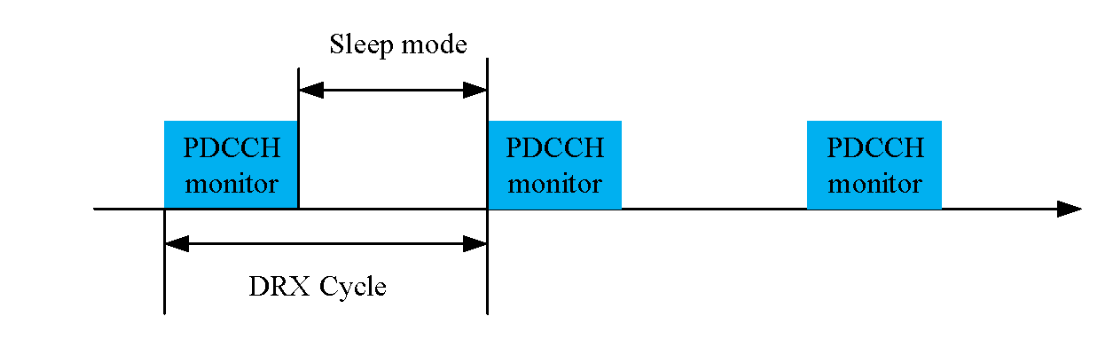
\includegraphics[width=\linewidth]{Pictures/Schematic diagram of DRX.png}
    \caption{Schematic diagram of DRX}
    \label{fig:5g-drx}
\end{figure}


%%%%%   CDRX in detail %%%%%%
    In CDRX \CAREPL{}{mode}, the Radio Resource Control (RRC) entity controls DRX operation by configuring the following parameters in the Media Access Control (MAC) layer \cite{3gpp_nr_nodate-3_38.331}:

\begin{itemize}
    \item \textit{drx-LongCycleStartOffset}: contains two parameters \textit{drx-LongCycle} and \textit{drx-StartOffset}. 
    The first \CAREPL{one}{parameter \textit{drx-LongCycle} } sets the \CAREPL{duration of DRX cycle and has values}{DRX cycle duration as a value} between 10 ms and 10.24 s. 
    \CAREPL{On the other hand,}{And} \CAREPL{drx-StartOffset}{the other one} defines the starting point \CAREPL{for}{of} the ON duration \CAREPL{and has the value in multiples of 1 ms}{*what do you mean?} (\CAREPL{see the illustration}{as illustrated} in \CAREPL{figure}{Fig.~} \ref{fig:basic-drx-operation}). 
    Note that the basic unit used in both DRX cycle and start offset is 1 ms which guarantees that \CAREPL{UE}{UEs} \CAREPL{will}{can} start the ON period at the beginning of a radio subframe.

\begin{figure}
    \centering
    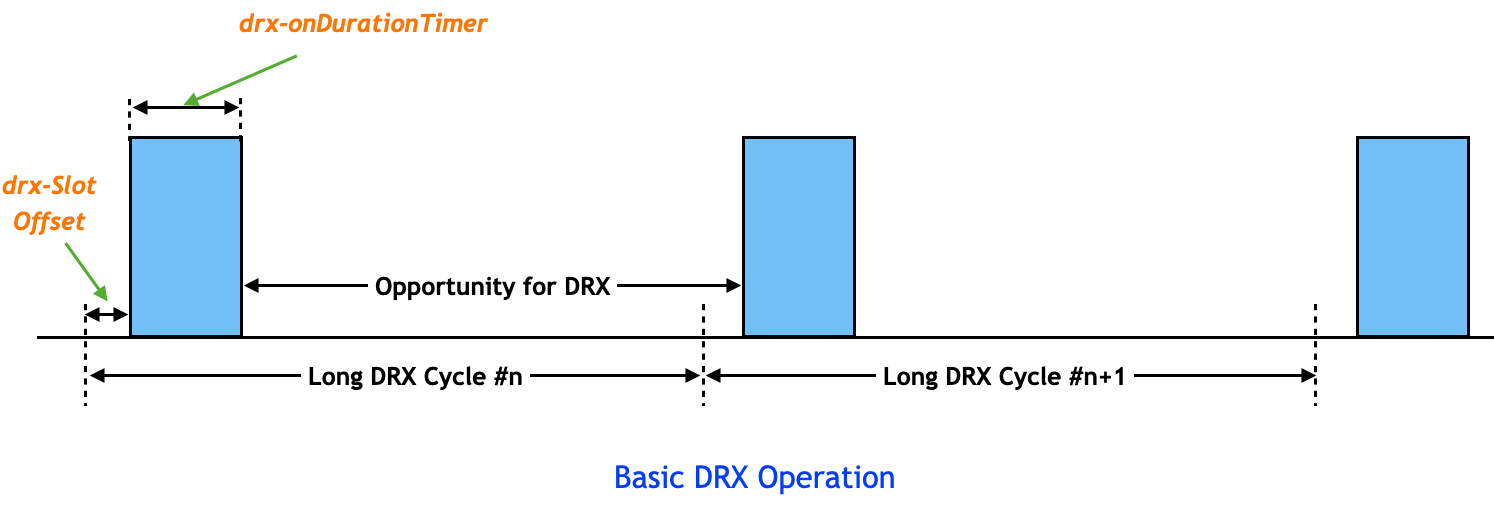
\includegraphics[width=\linewidth]{Pictures/Basic DRX Operation.png}
    \caption{Basic DRX Operation}
    \label{fig:basic-drx-operation}
\end{figure}
    
    \item \textit{drx-onDurationTimer}: a fixed timer at the beginning of every DRX cycle where UE is awake and listening for the control channel.
    When this timer expires, UE returns to sleep \CAREPL{}{mode} if there \CAREPL{are}{is} no \CAREPL{messages on} message transmitted in PDCCH. 
    \CAREPL{as shown in figure \ref{fig:basic-drx-operation}.}{} 
    This timer takes values in multiples of 1/32 ms (up to 1600 ms). The choice of the values of onDurationTimer is consistent with the slot clock that varies depending on sub-carrier spacing.
    \item \textit{drx-InactivityTimer}: a fixed timer \CAREPL{that starts}{} after a PDCCH \CAREPL{occasion}{} which indicates a new UL or DL transmission for the MAC entity. This timer overlaps the drx-onDurationTimer and cancels its effect. 
    In other words, the UE will continue monitoring \CAREPL{}{the} PDCCH and listen to the control information related to the upcoming messages even after the expiration of the drx-onDurationTimer. 
    Once the InactivityTimer times out and \CAREPL{if}{} there \CAREPL{are}{is} no \CAREPL{messages}{message} \CAREPL{on}{in the} PDCCH, UE will return to sleep \CAREPL{}{mode} as shown in figure~\ref{fig:5g-drx-InactivityTimer}. This timer takes values in multiples of ms (up to 2560 ms).
\begin{figure}
    \centering
    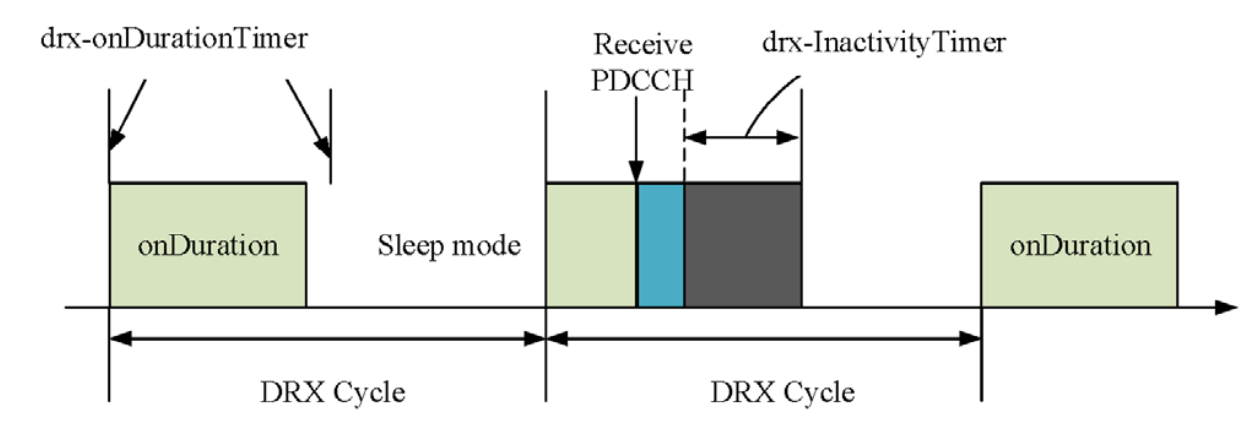
\includegraphics[width=\linewidth]{Pictures/Schematic diagram of drx-InactivityTimer.png}
    \caption{Schematic diagram of drx-InactivityTimer}
    \label{fig:5g-drx-InactivityTimer}
\end{figure}

    \item \textit{drx-ShortCycle}: \CAREPL{}{*definition first} UE can be configured with a shorter DRX cycle by setting this optional parameter. The duration of short DRX cycles can have values in the range between 2 and 640 ms.
    
    \item \textit{drx-ShortCycleTimer}: UE switches to operate in long DRX cycles after a number of short cycles with no activity \CAREPL{}{*not clear}. This number is defined by drx-ShortCycleTimer and has integer values up to 16.
\begin{figure}
    \centering
    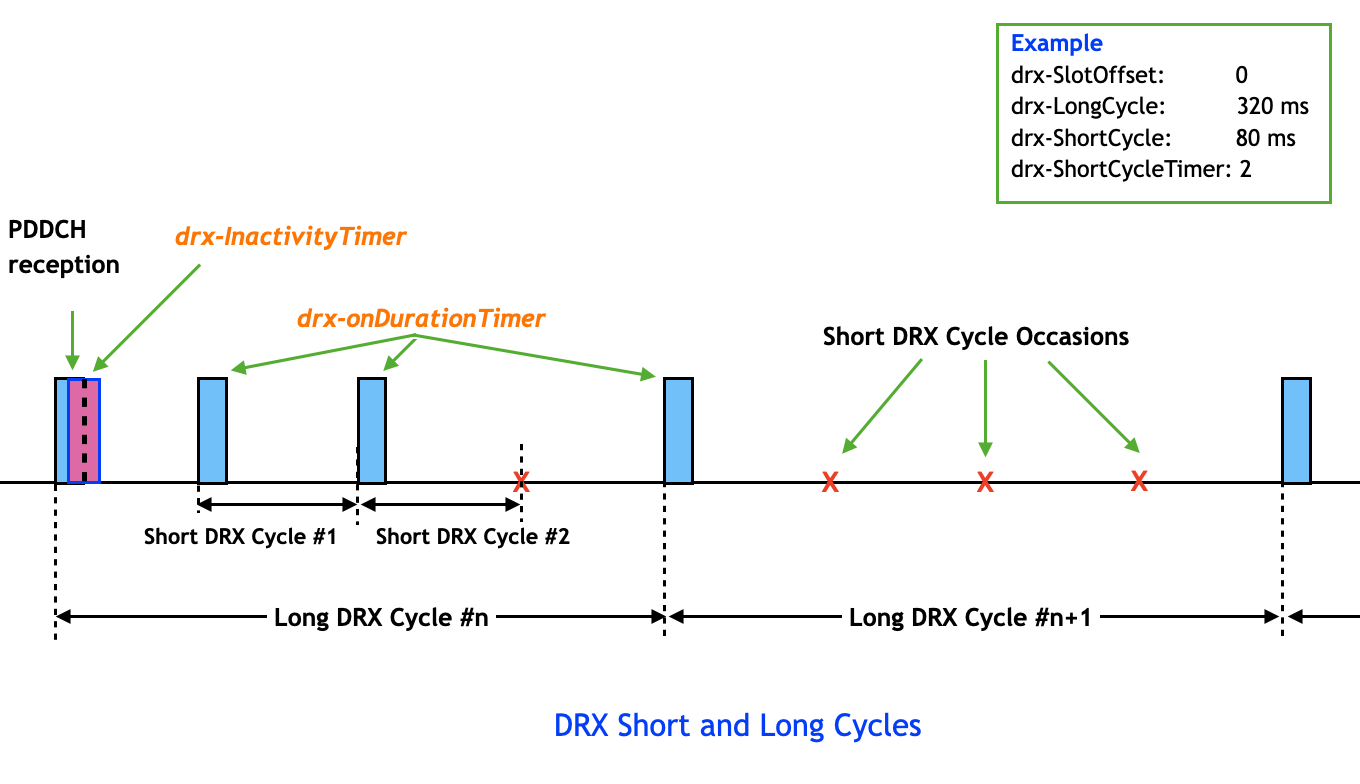
\includegraphics[width=\linewidth]{Pictures/Schematic diagram of drx-ShortCycleTimer.png}
    \caption{Schematic diagram of drx-ShortCycleTimer}
    \label{fig:5g-drx-ShortCycleTimer}
\end{figure}

\end{itemize}

%%%%%   Transition between CDRX and IDRX %%%%%%
A CDRX cycle starts with \CAREPL{}{an} ON period in which UE checks \CAREPL{}{* only one UE?} for control messages, i.e., DCI, on PDCCH channel. 
If UE has detected a packet arrival, it starts \CAREPL{the}{a} drx-InactivityTimer (This timer is restarted as long as UE still has an ongoing connection). 
Upon the expiry of the drx-InactivityTimer, UE enters a short DRX sleep cycle and later switches to long DRX after several iterations of short cycles as depicted in figure \ref{fig:5g-drx-ShortCycleTimer}. \CAREPL{}{*The figure does not correspond to what you give here.} 
\CAREPL{following}{After} a configured number of long DRX cycles the network releases UE's radio access context \CAREPL{}{* what do you mean "release"} and the UE enters to RRC\_Inactivity and later RRC\_Idle modes where it can benefit from an extended IDRX cycle \CAREPL{}{*citations}.



%%%%%   Intro to Paging %%%%%%
UEs in inactive/idle states do not have any active sessions. However, while sleeping, the UE is required to \CAREPL{ wake up in a periodic manner}{ be woken up periodically} to listen to paging messages, and short messages, i.e., System Information (SI) update notifications and emergency notifications (Earthquake/Tsunami Warnings (ETWS), Commercial Mobile Alerts (CMAS)). 
The paging procedure allows \CAREPL{the network to reach UEs}{*not clear} in inactive and idle modes. 
In RRC\_IDLE, the UE receives paging messages initiated by the core network. On the other hand, in RRC\_INACTIVITY, the paging control channel (PCCH) carries RAN-initiated paging messages. In NR, the same paging messages are sent over all beams and it is up to the UE to select the suitable beam by sensing the Synchronization Signal Blocks (SSBs).
\CAREPL{}{*Add your analysis here.}



%%%%%   How Paging works %%%%%%
Since mobile networks are synchronized communication systems, \CAREPL{UE can}{UEs need} \CAREPL{wake up}{ to be woken up} only at specific time instants, so-called paging occasion (PO). 
A PO consists of a set of PDCCH monitoring occasions located in the pre-configured pagingSearchSpace as specified in TS 38.213 \cite{3gpp_nr_2022-1_38.213}. 
Multiple POs form a Paging Frame (PF) that is \CAREPL{equal to}{*what do you mean "equal to", same length?} one Radio Frame (10 ms). 
In practice, a PO is transmitted over two channels, \CAREPL{PDCCH,}{the PDCCH} and an associated PDSCH \cite{esswie_power_2022} \CAREPL{channel}{}. 
UEs scan the configured PDCCH search space \CAREPL{and search}{} for a paging indication whose CRC is scrambled by \CAREPL{P-RNTI}{*mentioned before or not? if not, citation}. 
\CAREPL{Upon the detection of a paging indication the UE will decode the associated PDSCH looking for the pagingRecordList and to check if its UE\_ID is among the paged UEs.}{* I don't understand this sentence}

%%%%%   How UE knows which PF to listen to %%%%%%
\CAREPL{}{Each} UE monitors one PO per DRX cycle and \CAREPL{it}{} is able to precisely \CAREPL{calculate}{*calculate what to determine} and determine the System Frame Number (SFN) that carries its PF/PO \CAREPL{using the following parameters as specified in Clause 7 in TS 38.304 \cite{3gpp_nr_2022-10_38.304}:
 \begin{itemize}
     \item T: IDRX cycle of the UE (PagingCycle)
     \item N: number of total paging frames in T
     \item N$_{s}$: number of paging occasions for a PF
     \item UE\_ID: 5G-S-TMSI stored in USIM
 \end{itemize}
}{*Give the calculation procedure first.}
% -   Possible to go in detail about the calculation of PF/PO and the concepts of H-SFN, PTW, ...
% -   Adding illustrative figures to differentiate between SFN and H-SFN and how PF/PO occurs in them (see https://www.sharetechnote.com/html/Handbook_LTE_eDRX.html)


%%%%%   Details on the IDRX and the initial eDRX %%%%%%
The value of T comes from two different sources. The first is defaultPagingCycle which is broadcasted by the gNB to all UEs through system information messages (SIB). The second source is UE-specific cycle defined by RRC and/or upper layers. \CAREPL{}{*The introduction of parameters can be integrated into this paragraph. } 
The UE sets the IDRX cycle to the minimum between these two values \CAREPL{}{*How}. \CAREPL{PagingCycle is an integer number of radio frames}{* I don't understand} and has a maximum value of rf256 $\approx2.56 s$. 
This upper bound was later extended and specified in Rel-17 to 10.24 s which corresponds to 1024 radio \CAREPL{frame,}{frames,} \CAREPL{}{*transmission time?} i.e., the maximum allowed SFN.

%%%%%   Introducing eDRX in RedCap %%%%%%
In the RedCap \CAREPL{study phase}{studies}, \CAREPL{a further extension of the IDRX cycle, beyond 10.24 s,}{an IDRX cycle beyond  10.24s} was discussed. 
\CAREPL{The main objective was to study the potential power-saving gain and the possible mechanisms to achieve this extension.}{* I don't understand. You mean to save energy or to achieve this length?} 
The proposed approach is to reuse the applicable parts of \CAREPL{}{the} eDRX mechanism \CAREPL{used}{} in LTE RAN, including the \CAREPL{usage of}{} Hyper-SFN (H-SFN) and \CAREPL{}{the} Paging Time Window (PTW), see clause 7.4 in TS 38.304 \cite{3gpp_nr_2022-10_38.304} for more details. 
This mechanism was \CAREPL{originally}{initially} designed for NB-IoT and LTE-M to \CAREPL{allow the extension of}{extend the} long eDRX cycles up to a few hours, \CAREPL{. The upper bound of eDRX cycles is limited}{which is upper bounded} by the upper value of the H-SFN (1048576 radio frame $\approx$2.91 hrs) \CAREPL{and it is supported by the 5G core only for RRC\_IDLE since NB-Iot and LTE-M are connected to it in the non-standalone architecture.}{* redo this sentence}

 %%%%%   What is the performance enhancement?   %%%%%%
The evaluation results \CAREPL{submitted}{obtained} by several vendors \CAREPL{and}{are} summarized in Annex E.1 in TR 38.875 \cite{3gpp_study_2021_38.875} \CAREPL{present a}{. A} clear power-saving enhancement \CAREPL{of}{by} extending eDRX beyond 10.24s \CAREPL{}{can be observed}. 
The results \CAREPL{showed a power-saving in the range of 80-90$\%$}{suggested an 80-90\% power saving} \CAREPL{when using}{with} a DRX cycle of 10485.76 s compared to the normal IDRX setting of 2.56 s. 
The study also showed \CAREPL{that UEs start to experience}{} a clear power-saving gain when \CAREPL{}{the} eDRX cycle is \CAREPL{in the range}{extened} from 10.24 seconds up to a few minutes. 
This reduction in energy consumption may substantially extend the battery lifetime of \CAREPL{the UE}{UEs} which is \CAREPL{an}{} important \CAREPL{requirement}{} for some use cases like industrial wireless sensors \CAREPL{}{*citations, it would be better if you can give several examples}.
 
 %%%%%   what is the recommended configuration to be specified in WI   %%%%%%
 Based on the \CAREPL{aforementioned advantages}{advantages mentioned above}, \CAREPL{it was decided in the recommendations of the design of}{} RedCap devices \CAREPL{}{are recommended} to support an extended DRX cycle of 10485.76 s in both RRC\_IDLE and in RRC\_INACTIVE states \CAREPL{}{*citations}. 
 The \CAREPL{full}{} details of the mechanisms and feasibility of this extension are still \CAREPL{ongoing topics and}{} need further review with other 3GPP groups, namely, SA2, CT1, and RAN4. \CAREPL{}{list some efforts and their results.}



\subsection{RRM relaxation for stationary devices}
\label{sec:5-2}


% Main Question this subsection tries to answer:
%     -   What kind of measurements does the UE perform? and why?
%     -   What is the problem with this system of work? (Unnecessary for stationary)
%     -   What is the solution? (RRM measurement relaxation)
%     -   How this solution works? (Triggers and mechanisms)
%     -   What is special in RedCap and what was standardized?

%%%%%   Few words about mobility and RRM meausrements in 5G?   %%%%%%
\CAREPL{One of the fundamental characteristics of cellular networks is the support of mobility.}{} 
Mobility management  \CAREPL{encapsulates}{plays an important role in cellular networks, which consists} a list of operations \CAREPL{,}{} including \CAREPL{,}{} measurements, cell selection/(re)selection \CAREPL{,}{} and handover. 
\CAREPL{Both gNB and UE cooperate to achieve these RRM-related operations that are done seamlessly to the end user.}{* I don't understand this sentence} 
\CAREPL{gNB will}{gNBs} configure UEs \CAREPL{with the required parameters}{} to achieve intra-frequency, inter-frequency, and inter-RAT cell selection/re-selection following the requirements specified in TS 38.133 \cite{3gpp_nr_2022-11_38.133}. 
The configuration includes defining parameters like the frequency points, the periodicity, and the number of measured samples. 
UEs \CAREPL{will}{periodically} report to the gNB the values of reference signal received power (RSRP), reference signal received quality (RSRQ), and Signal-to-Interference-and-Noise Rate (SINR) measured from both the serving and neighboring cells. 
\CAREPL{Such}{These} RRM measurements \CAREPL{will}{can} guarantee that \CAREPL{the}{each} UE \CAREPL{is camping}{connects} to the best available cell and ensure a good quality of communication.
%%%%%   What is the problem?  %%%%%%

In 5G \CAREPL{network}{networks}, mobility management is a challenging task, \CAREPL{especially, with the introduction of new technologies such as Beamforming}{*citation, I don't think beamforming is a new technique for 5G networks.}. 
In order to connect to the best available Beam, UE needs a very precise evaluation of all possible beams. 
Even though these measurements are essential to achieve the best performance, they are in some scenarios either unnecessary or not optimized for the mobility profile of the UE. 
This can lead to excessive power consumption that can drain the UE battery. 
In some use cases such as industrial wireless sensors and Video Surveillance, UEs are more \CAREPL{or less}{} stationary and the required RRM measurements can be relaxed.

%%%%%   What is the solution? (RRM measurement relaxation)    %%%%%%
\CAREPL{Therefore,}{*why therefore?} \CAREPL{already}{} in Rel-16, 3GPP has defined a new power-saving technique to mitigate the aforementioned problem of unnecessary measurements. It was a suggested feature in the study on UE power-saving in NR \cite{3gpp_study_2019_38.840}.

%%%%%   What is RRM measurement relaxation?    %%%%%%
 RRM measurements relaxation aimed to specify less frequent UE-specific measurements that adapt the mobility state of the terminal. 
 This feature can be initiated once the UE fulfills some criteria, so-called triggers. 
 RRM Measurement relaxation triggers are configured \CAREPL{to the UE}{at UEs} by the serving cell through SIB messages. 
 In Rel-16, \CAREPL{two triggers}{* you mentioned two triggers here, why there are four subsections} were primarily specified: \textit{UE with low mobility} and \textit{UE not at cell edge}. According to TS 38.804 \cite{3gpp_study_nodate-4_38.804}, they are defined as followed:\\

 %%%%%   Triggering Criteria    %%%%%%
\subsubsection{\textbf{Criterion for UE with low mobility}} This trigger \CAREPL{defines}{is for} UEs \CAREPL{that are}{} in low-mobility state\CAREPL{. It}{, which} is based on the fact that the level of RSRP does not dramatically change when UE is moving slowly. 
\CAREPL{UE will monitor the variations in RSRP level received from}{UEs adapt themselves in RSRP level to} the serving cell\CAREPL{. This condition}{, which} can be \CAREPL{translated in the following formula:}{formulated as fokkows:}
\begin{equation}
\CAREPL{Srxlev_{Ref}-Srxlev<S_{SearchDeltaP}}{*subscripts are too long}
\label{equ:low-mobility-criterion}
\end{equation}
\CAREPL{Where $Srxlev$ and $Srxlev_{Ref}$ are the current and reference Cell selection Rx level value (in dB) and these values are directly driven from the measured RSRP level (See clause 5.2.3.2 in TS 38.804 \cite{3gpp_study_nodate-4_38.804}).}{* I don't understand this sentence} 
$S_{SearchDeltaP}$ specifies the threshold (in dB) \CAREPL{on}{of} \CAREPL{Srxlev}{$Srxlev$} variation. 
The value of $Sexlev_{Ref}$ is updated \CAREPL{with the current level}{} in three conditions:
\begin{enumerate*}
    \item After selecting or re-selecting a new cell;
    \item if the UE is moving toward the center of the cell (i.e., $Srxlev-Srxlev_{Ref}<0$), and
    \item if the condition in equ. \ref{equ:low-mobility-criterion} has not been met for a period of $T_{SearchDeltaP}$.
\end{enumerate*}

We see that the level of "low mobility" is not strict and is defined by choosing the value of $T_{SearchDeltaP}$ and  $S_{SearchDeltaP}$ and it is up to the operator to set these parameters.\\

\subsubsection{\textbf{Criterion for \CAREPL{UE}{UEs} not at cell edge}} This trigger \CAREPL{defines}{is for} UEs that are located not at the edge of the serving cell. 
It \CAREPL{compares the }{allows UEs compare their} current level of RSRP with a configured threshold $S_{SearchDeltaP}$, \CAREPL{communicated to the UE via SIB messages:
\begin{equation}
Srxlev>S_{SearchThresholdP}
\label{equ:not-at-the-edge-criterion}
\end{equation}
}{* What do you mean here}
If \CAREPL{the level of the measured}{the UE's} RSRP \CAREPL{}{level} (and subsequently $Srxlev$) is greater than a \CAREPL{certain}{*prefixed?} threshold ($S_{SearchThresholdP}$), the UE is considered close to the cell center and less likely to attach to another neighbor cell. 
\CAREPL{This permits the UE to relax the mobility management setting by having less frequent RRM measurements and saving more power.}{*how?}

\CAREPL{}{* Please reconsider the storyline from here}

Due to the low mobility property of some RedCap use cases, new triggers for RRM measurement relaxation can be introduced. Several enhancements were discussed in the study phase including:
\begin{enumerate}
    \item Introduction of stationary UE state,
    \item Use beam measurements to determine UE mobility state,
    \item Definition of the mobility state in the subscription information, i.e., in USIM.
\end{enumerate}
%%%%%   Enhancement in RedCap   %%%%%%
However, only two triggering criteria were later specified for RedCap devices:\\
\subsubsection{\textbf{Criterion for a stationary RedCap UE}} This trigger defines RedCap UEs that are in a stationary state. It follows the same approach used in the low mobility criterion by sensing the variation of the level of RSRP measured from the serving cell:
\begin{equation}
Srxlev_{RefStationary}-Srxlev<S_{SearchDeltaP-Stationary}
\label{equ:stationary-criterion}
\end{equation}
UE must sense the level of the received signal, and according to the parameters (duration and threshold) defined by the network, RRM relaxation mode will be triggered. 

\subsubsection{\textbf{Criterion for a stationary RedCap UE not at cell edge}} This trigger combines the two previous criteria and triggers an intensive RRM measurement relaxation once the UE fulfills both "Stationary" and "no at cell edge" conditions. \\


%%%%%   What are the methods of RRM relaxation? (After the trigger)    %%%%%%
Once the UE fulfills any of the aforementioned criteria it can start the RRM relaxation operation. Many approaches to perform RRM measurements relaxations have been discussed during the study phase of RedCap and in previous work items of 3GPP \cite{3gpp_ue_2019_R2-1912335,3gpp_rrm_2019_R2-1912334,1912531_R2-1912531}, including:
\begin{enumerate}
    \item Increase the interval between RRM measurement;
    \item Reduce the number of neighboring cells to be measured;
    \item Reduce the number of measured carrier frequencies; and
    \item Reduce the number of monitored reference signals.
\end{enumerate}
The methodology that has been adopted so far in NR is based on increasing the RRM measurements cycle time. This is done by skipping some measurement occasions as illustrated in figure \ref{fig:rrm-relaxation}. UE has to perform RRM measurements every N DRX cycle where N is a scaling factor that is communicated to UE as defined in TS 38.133 \cite{3gpp_nr_2022-11_38.133}.

\begin{figure}
    \centering
    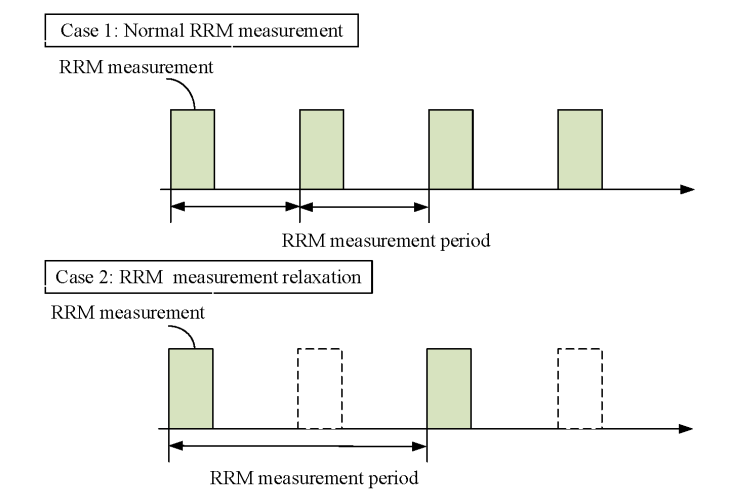
\includegraphics[width=\linewidth]{Pictures/RRM measurement relaxation.png}
    \caption{Example of RRM measurement relaxation}
    \label{fig:rrm-relaxation}
\end{figure}

%%%%%   What are the positive and negative impacts?      %%%%%%
Different companies have contributed to the study item of RedCap \cite{3gpp_study_2021_38.875} by evaluating and analyzing the gain and impact of using RRM measurement relaxation. One source \cite{3gpp_tp_2021_R2-2100459} has shown a power-saving gain of $3.6\% - 26.6\%$ when increasing the RRM measurement cycle 4 times with different UE states of idle/inactive and connected modes. This gain comes at the expense of a slight increase in the handover failure rate of $0.26\%$.
Another contribution from Huawei \cite{3gpp_further_2020_R2-2009116} showed an enhancement of $25\%$ in UE power saving by increasing RRM measurement intervals from a few seconds to 1 hour. This study also showed a potential gain of $13.54-16.25\%$ in UE power-saving if the number of measurement of SSBs blocks is reduced by $62.5-75\%$.
Ericsson on the other hand, claimed that the power saving gained by increasing the measurement intervals beyond one hour (the maximum possible in NR Rel-16) is insignificant \cite{3gpp_redcap_2020_R2-2009620}. Their conclusion was based on the evaluation of UEs in both RRC\_IDLE or RRC\_INACTIVE states.

%   

\section{RedCap impact on network performance}
\label{sec:6-redcap-impact}


%%%%%   Some preamble about the importance of system evaluation %%%%%%
An important objective of the study of RedCap \CAREPL{was}{is} to analyze and evaluate \CAREPL{the potential impact and performance degradation arising from the limitation of RedCap devices.}{*what do you mean?} 
The proposed features, presented in Sections \ref{sec:4-complexity-reduction} and \ref{sec:5-power-saving}, have great \CAREPL{advantages}{*potentials?} in terms of lowering the device cost/complexity and enhancing the UE battery lifetime. 
\CAREPL{However, an impact on system performance is expected, and therefore more detailed and quantitative evaluation is required to estimate the degradation and enable some functionalities to mitigate or limit it. }{* I don't understand}
Two main performance indicators were largely discussed in \cite{3gpp_study_2021_38.875}: Coverage Loss and Network Capacity/Spectral-Efficiency. We present in the following subsections the evaluation methodologies agreed on and the final results/takeaway.  

\subsection{Coverage \CAREPL{Analysis}{Loss}}
\label{sec:6-1}
% -   What are the potential sources of the problem?
% -   What are the metrics used to assess the coverage? (MIL, MPL, MCL) 
% -   What are the used channels/msgs? (PDCCH, PDSCH, ...) 
% -   what are the propagation scenarios? (Urban, Rural, ...)
% -   What are the steps to perform the evaluation? (Two steps: LLS and MIL calc)
% -   What are the results and final takeaway?
% -   What are the proposed coverage recovery techniques?


%%%%%   The potential source of problem     %%%%%%
RedCap devices are expected to experience \CAREPL{a coverage loss}{coverage losses} due to some of the complexity reduction features. 
\CAREPL{The}{Their} main impact on coverage \CAREPL{is coming from the following considerations:}{are listed as follows:}
\begin{itemize}
    \item Reduced number of \CAREPL{UE}{} Rx \CAREPL{Antenna}{antennas}: This \CAREPL{feature will cause}{causes} a loss in spatial diversity which can affect the quality of the received signal and subsequently \CAREPL{the coverage}{causes coverage losses.} 
    \item \CAREPL{UE bandwidth Reduction: RedCap device will lose in frequency diversity where it will be limited to operate on a smaller bandwidth. This can lead to a coverage loss in some propagation scenarios.}{*I don't understand this point. Lack of spectrum diversity may cause more collisions, but why coverage loss? Please add some citations to justify this point.}
    \item \CAREPL{Antenna efficiency loss: the smaller size of RedCap device in some use cases such as wearables will affect the antenna gain. The estimated coverage loss is around 3 dB.}{* Because antennas are in small size? Please justify it with some citations}
\end{itemize}

%%%%%   The metric to estimate the loss     %%%%%%
\CAREPL{To analyze the coverage performance, link budget evaluation was used.}{The link budget evaluation is a widely used method to analyze the coverage performance.} 
\CAREPL{There exist several formulas used to calculate link budget such as, Maximum Path Loss (MPL), Maximum Coupling Loss (MCL), Maximum Isotropic Loss (MIL). Both MPL and MIL include the antenna gains. 
However, in consistence with the agreement of the work item of NR coverage enhancements \cite{3gpp_study_nodate-3_38.830}, it was decided to use MIL. MIL is used to derive the relative differential values between channels and identify the bottlenecks.\\}{*Please reconsider the storyline here}

\CAREPL{MIL = Total transmit power – Receiver sensitivity – Tx loss – Rx loss + gNB antenna gain + UE antenna gain.\\}{*Make it an equation or integrate it into the last paragraph.}

More details on the link budget template can be found in Annex A.3 of \cite{3gpp_study_nodate-3_38.830}. \textcolor{red}{We can add some figure like \ref{fig:MIL-diagram}}

\begin{figure}
    \centering
    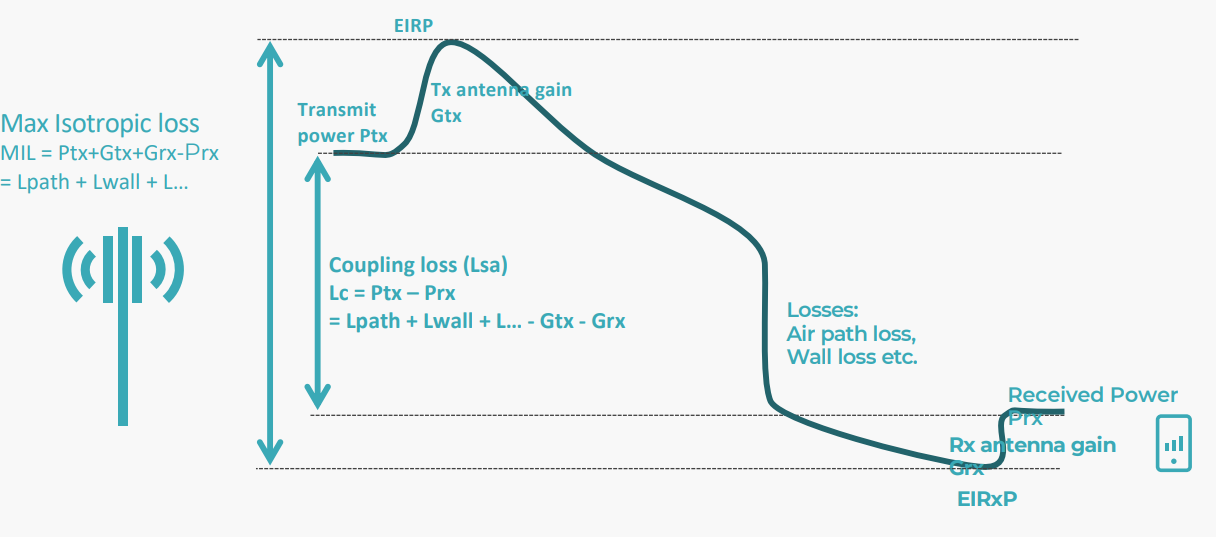
\includegraphics[width=\linewidth]{Pictures/Link budget representation.png}
    \caption{Representation Maximum link budget}
    \label{fig:MIL-diagram}
\end{figure}

%%%%%   The metric to estimate the loss  (MIL)   %%%%%%
\CAREPL{Since any of the physical channels can limit the coverage of UE,}{*why?} different types of control and data channels along with the random-access channels were used to carry out the link budget evaluation. A list of the main channels and the associated messages are given in table \ref{table:coverage-evaluation-physical-channels}
\begin{table}
\centering
\caption{Physical channels used in coverage evaluation}
\begin{tabular}{| m{0.08\linewidth}  m{0.8\linewidth}|} 
 \hline
    \textbf{Name}  &  \textbf{Description} \\
\hline
    PRACH & Physical Random Access Channel is used by UE to send a preamble in order to initiate the connection\\
\hline
    PBCH & Physical Broadcast Channel carries system information messages and the primary/secondary synchronization signals PSS/SSS\\
\hline
    PDCCH & Physical DL Control Channel conveys DCI to UEs e.g., scheduling information \\
\hline
    PDSCH &  Physical DL Shared Channel is used to carry UE data on the DL\\
\hline
    PUCCH &  Physical UL Control Channel is used to send feedback to gNB e.g., acknowledgments and channel-state reports\\
\hline
    PUSCH &  Physical UL Shared Channel is used to carry UE data on the UL\\
\hline
    Msg2 &  Message 2 or Random Access Response (RAR) is an indication from the gNB about the reception of UE preamble and carries the uplink grants for Msg.3\\
\hline
    Msg.3 &  Message 3 is used by UE to transmit RRC message(e.g, RrcRequest) and includes information about the device identity and capabilities\\ 
\hline
    Msg4 &  Message 4 or Contention Resolution message confirms that the gNB has correctly identified the UE, and resolved the possible contention and it transfers the UE to RRC\_connected state\\
\hline
\end{tabular}
\label{table:coverage-evaluation-physical-channels}
\end{table}

%%%%%   The Scenario Parameters      %%%%%%
\CAREPL{The same coverage evaluation assumptions of the Rel-17 Coverage enhancement SI \cite{3gpp_study_nodate-3_38.830} were reused in the RedCap evaluation.}{*not mentioned before?} 
Three propagation scenarios have been studied: Rural and Urban in \CAREPL{FR1}{*citation} and Indoor in \CAREPL{FR2}{*citation}. 
A list of the main parameters of each of these scenarios is summarized in table \ref{table:scenarios-parameters}\CAREPL{. Table \ref{table:scenarios-parameters} 
}{, which} also includes the common assumptions and the specifications used to differentiate between RedCap and reference NR devices.
\begin{table}
\centering
\caption{Simulation Assumptions used in coverage evaluation}
\begin{tabular}{|m{0.2\linewidth} | m{0.12\linewidth} |  M{0.15\linewidth}| M{0.15\linewidth} | M{0.15\linewidth}|} 
 \hline
    \multicolumn{2}{|c|}{\textbf{Scenario Parameters}}  & \textbf{Rural}  &  \textbf{Urban} & \textbf{Indoor} \\

\hline
    \multicolumn{2}{|c|}{Carrier frequency} & 0.7 GHz & 2.6 GHz and 4 GHz  & 28 GHz\\
\hline
    \multicolumn{2}{|c|}{Sub-carrier spacing} & 15 kHz & 30 kHz & 60 kHz\\
\hline
    \multicolumn{2}{|c|}{Duplexing} & FDD & \multicolumn{2}{c|}{TDD}\\
\hline
   \multicolumn{2}{|c|}{Delay Spread} &  \multicolumn{2}{c|}{300 ns} & 30 ns\\
\hline
    \multicolumn{2}{|c|}{gNB TX chains} & 2 & 4 & 2\\
\hline
    \multicolumn{2}{|c|}{gNB RX chains} & 2 & 4 & 2\\
\hline
    \multicolumn{2}{|c|}{UE TX chains} & \multicolumn{3}{|c|}{1}\\
\hline

    \multirow{2}{*} {UE RX chains} & Ref. NR & 2  & 4 & 2 \\
    \cline{2-5}
    &   RedCap  &  \multicolumn{3}{|c|}{1 or 2}  \\
\hline
    \multirow{2}{*} {UE bandwidth} & Ref. NR & 20 MHz & \multicolumn{2}{|c|}{100 MHz} \\
    \cline{2-5}
    &   RedCap  &  \multicolumn{2}{|c|}{20 MHz} & 50 MHz or 100 MHz  \\
\hline
    \multicolumn{2}{|c|}{UE speed profile} & \multicolumn{3}{|c|}{3 km/h}\\
\hline
    \multicolumn{2}{|c|}{UE antenna correlation} & \multicolumn{3}{|c|}{low}\\
\hline
\end{tabular}
\label{table:scenarios-parameters}
\end{table}

%%%%%    What are the steps to perform the coverage evaluation?  %%%%%%
For both RedCap and reference UEs, the target performance requirements of \CAREPL{each of the}{} physical channels/signals are defined, i.e., min throughput, block error rate (BLER), no. of HARQ re-transmission, etc. 
After that, the coverage evaluation to determine if RedCap device requires coverage recovery \CAREPL{is}{can be} carried out \CAREPL{ following}{by adopting the} three main steps \CAREPL{}{as follows}:
\begin{enumerate}
    \item  Perform a Link-level Simulation (LLS)  \CAREPL{to figure out the required SNIR that meets the performance target of each of the examined physical channels. }{* I don't understand}
    \CAREPL{T}{Note that t}he simulation is done \CAREPL{with respect to}{using} the parameters defined in table \ref{table:scenarios-parameters}.
    \item Use the results of the LLS (i.e., SINR levels) to calculate the link budgets MILs.
    \item Once the MIL \CAREPL{levels}{level} of all \CAREPL{different}{} channels are calculated, \CAREPL{the amount of}{*why} required coverage recovery is identified by the \CAREPL{link budget (MLI)}{*?} of the bottleneck channel for the reference NR device within the same \CAREPL{deployment}{} scenario. The bottleneck channel is the physical channel that has the lowest MIL.
\end{enumerate}
In Summary, \CAREPL{}{physical channels used by} \CAREPL{a}{} RedCap \CAREPL{UE}{UEs} \CAREPL{that has physical channels that experience}{ are normally with} a MIL worse \CAREPL{than}{compared to} the bottleneck channel of a reference NR device in \CAREPL{the same propagation scenarios}{same physical environment}. \CAREPL{needs to compensate for the difference.}{* I don't understand}
\CAREPL{}{*Justify why}

%%%%%    Summary of the results of coverage evaluation  %%%%%%
Different companies have contributed to RedCap study by performing the link budget analysis. \CAREPL{The results of the simulation}{Simulation results} of different sourcing companies can be found in Annex C of TR 38.875 \cite{3gpp_study_2021_38.875} and in \cite{3gpp_fl_2022_R1-2009293}. As a conclusion of coverage evaluation of RedCap devices the following outcomes are made:
\begin{itemize}
    \item In FR1, for both Rural and Urban scenarios, due to the \CAREPL{size limitation}{limited size} of RedCap device\CAREPL{}{,} a reduced antenna efficiency of 3 dB is expected. 
    As a result, both PUSCH and Msg3 \CAREPL{experience}{have} a MIL level that is less than the bottleneck channel of the reference NR UE and a coverage recovery is needed. 
    However, \CAREPL{the}{} other UL physical channels do not require coverage compensation since they have a MIL level higher than the bottleneck channel. 
    For the DL physical channels, the coverage is dependent on the frequency bands (i.e., 0.7 GHz, 2.4 GHz, or 4 GHz) and the assumptions of the DL Power Spectral Density \CAREPL{(DL PSD)}{(PSD)}. The most affected signals are Msg2 and Msg4 with a potential degradation of 6 dB, especially\CAREPL{,}{} for RedCap UEs with 1 Rx. This coverage degradation can be mitigated by using the \CAREPL{existing}{}  Transport Block Size (TBS) scaling technique\CAREPL{}{. *better with a citation}
    \item In FR2 \CAREPL{at}{with} mm Waves, \CAREPL{the antennas have a small form and the RedCap device size will not affect the antenna efficiency.}{*reconsider this sentence}
    Therefore, the MIL levels of UL channels are equivalent to the ones of the reference NR UE. \CAREPL{and}{Thus,} no coverage recovery is needed\CAREPL{ on the UL.}{.} 
    \CAREPL{On the other hand}{However,} for the DL channels, a coverage recovery in the range [2-3 dB] is needed for PDSCH, for RedCap UE with 50 MHz BW and 1Rx.\CAREPL{}{*citations to justify it}
\end{itemize}

%%%%%    Coverage recovery techniques  %%%%%%

\CAREPL{Regarding the coverage recovery, no new solutions were specified for RedCap UEs as a result of the work item. }{* I don't understand} 
However, RedCap devices \CAREPL{are assumed to reuse}{ can use} the existing UL coverage enhancement solutions (e.g., PUSCH repetition)  specified in the Rel-17 NR Coverage Enhancement WI (NR\_cov\_enh) \cite{3gpp_study_nodate-3_38.830} \CAREPL{}{to ...}. 
Other techniques from Rel-15/16, such as TBS scaling, are also available for RedCap UEs.






\subsection{Capacity Analysis}
\label{sec:6-2}

%%%%%    The source of the problem of capacity?  %%%%%%
Similar to the coverage performance, the introduced complexity reduction features of RedCap devices are expected to negatively affect the overall system capacity. 
Simplifications, such as reducing the number of antennas and the modulation order, have a direct impact on the spectral efficiency and consequently \CAREPL{}{may reduce} the system capacity. 
Therefore, \CAREPL{a quantitative evaluation of this impact has}{evaluations need} to be done before approving these features.

%%%%%    The agreed simulation assumptions  %%%%%%
A system-level simulation (SLS) must be conducted to evaluate the \CAREPL{system's performance}{*detials}. 
\CAREPL{It was agreed to re-use}{And} the simulation assumptions \CAREPL{from}{defined in} TR 38.802 \cite{3gpp_study_nodate-2_38.802} \CAREPL{}{can be used} as a baseline. 
Some additional modifications were proposed for the study case of RedCap \CAREPL{}{to ...}. 
A list of the main simulation parameters for both RedCap and Reference NR devices \CAREPL{is}{are} given in Table \ref{table:sls-assumption}. 
The rest of the simulation parameters can be found in Table 6.4-1 and Table D-1 in \cite{3gpp_study_2021_38.875}. 
Several traffic models \CAREPL{were used}, including full buffer traffic and bursty traffic such as File Transfer Protocol Model 3 (FTP3) and Instant Messaging (IM) \CAREPL{,}{are also used in simulations.} \CAREPL{where each of these models}{Each of them} is characterized by different packet sizes and inter-arrival time \CAREPL{}{to ...}. 
The overall Resource Utilization (RU) in the cell is related to the number of UEs and the traffic model used. The complexity reduction features of RedCap devices are consistent with the one presented in Section \ref{sec:4-complexity-reduction}. The metric used to evaluate the system performance is the average spectral efficiency (SE) and it is defined as follows:
\begin{equation}
\textrm{SE}=\frac{\textrm{cell average throughput (Mbps)}}{\textrm{cell bandwidth (MHz)}\times\textrm{RU}}
\label{equ:spectral-efficiency}
\end{equation}
\CAREPL{}{*check the storyline later}


\begin{table}
\centering
\caption{Assumptions for SLSs}
\begin{tabular}{|p{0.23\linewidth}| p{0.33\linewidth} |  p{0.33\linewidth}|} 
 \hline
    \textbf{Parameters}  & \textbf{RedCap UE}  &  \textbf{Reference UE}\\
\hline

\begin{itemize}[leftmargin=0,label={}]
        \item Scenarios
    \end{itemize}  & 
    \multicolumn{2}{|p{0.66\linewidth}|}{
    \begin{itemize}[leftmargin=*]
        \item Dense Urban: 2.6 GHz and 4 GHz (TDD)
        \item Indoor: 28 GHz (TDD)
    \end{itemize} 
    }\\
\hline

    \begin{itemize}[leftmargin=0,label={}]
        \item Traffic Model
    \end{itemize}  & 
    \begin{itemize}[leftmargin=*]
        \item Full buffer (optional)
        \item FTP model 3
        \item IM traffic model
    \end{itemize}   &

    \begin{itemize}[leftmargin=*]
        \item Full buffer (optional)
        \item FTP model 3
    \end{itemize}   \\

\hline
    \begin{itemize}[leftmargin=0,label={}]
        \item Traffic load
    \end{itemize}  & 
    \multicolumn{2}{|p{0.66\linewidth}|}{
    \begin{itemize}[leftmargin=*]
        \item Full buffer (optional): 10 users per cell
        \item Other traffic models: low ($<30\%$) and medium ($30-50\%$) resource utilization
    \end{itemize} 
    }\\
\hline
    \begin{itemize}[leftmargin=0,label={}]
        \item Scheduled BW
    \end{itemize}   & 
    \begin{itemize}[leftmargin=*]
        \item 20 MHz in FR1
        \item 50 or100 MHz in FR2
    \end{itemize}   &
    
    \begin{itemize}[leftmargin=*]
        \item 100 MHz for FR1/FR2
        
    \end{itemize}   \\
\hline
    \begin{itemize}[leftmargin=0,label={}]
        \item Max modulation order
    \end{itemize}  & 
    \begin{itemize}[leftmargin=*]
        \item 64QAM for DL
        \item 16QAM for UL
    \end{itemize}   &
    
    \begin{itemize}[leftmargin=*]
        \item 254QAM for DL
        \item 64QAM for UL
    \end{itemize}   \\
\hline

    \begin{itemize}[leftmargin=0,label={}]
        \item UE Rx / MIMO layers
    \end{itemize}  & 
    \begin{itemize}[leftmargin=*]
        \item 1Rx or 2Rx
    \end{itemize}   &
    
    \begin{itemize}[leftmargin=*]
        \item 4Rx in FR1
        \item 2Rx in FR2
    \end{itemize}   \\
\hline
    \begin{itemize}[leftmargin=0,label={}]
        \item  RedCap UE ratios
    \end{itemize}  &  
    \multicolumn{2}{|p{0.66\linewidth}|}{
    \begin{itemize}[leftmargin=*]
        \item $0\%,\: 25 \%,\: 50 \%,$ or $100 \%$ of the UEs in the cell are RedCap devices
    \end{itemize} 
    }  \\
\hline

\end{tabular}
\label{table:sls-assumption}
\end{table}

%%%%%    The agreed SLS results  %%%%%%
The results of the SLS from different companies are gathered in Tables D-1 to D-25 in Annex D of \cite{3gpp_study_2021_38.875}. 
The evaluations \CAREPL{cover}{covered} different combinations of the parameters presented in Table \ref{table:sls-assumption}. 
The outcome of the capacity and spectral efficiency evaluation can be summarized \CAREPL{in the following}{as follows}:

\begin{itemize}
    \item In the case where both types of UEs have bursty traffic, FTP3 is assumed for eMBB users and IM traffic for RedCap devices. The results show that introducing RedCap devices will have a marginal impact on the \CAREPL{user}{} throughput of other eMBB UEs and the overall system capacity \CAREPL{}{*more detials}. 
    It is worth noting that given the considered traffic models, the RedCap devices generate 0.1 MB payload every 2 s (400 kbps) while eMBB devices have 0.5 MB payload every 200 ms (20 Mbps). 
    \CAREPL{This}{It} means that the generated load of RedCap devices is very limited even when a \CAREPL{high ratio of RedCap devices}{*what do you mean} is connected to the cell. 
    The IM traffic model is only valid for the use cases of video surveillance and industrial wireless sensors where the exchanged traffic is dominated by the UL \CAREPL{}{*maybe, but why?}.
    \item \CAREPL{In the case where both devices have an FTP3 traffic model. This evaluation is suitable when RedCap devices are wearables and has more traffic on the DL.}{In wearable device use cases, both types of devices have the FTP3 traffic model and the amount of data in the DL is much higher than in the UL.} 
    The \CAREPL{test} results \CAREPL{vary}{} between \CAREPL{the sourcing}{} companies \CAREPL{}{are quite different}. 
    On one hand, Nokia stated that the throughput of eMBB device is not affected by the introduction of RedCap device. On the other hand, Huawei/HiSilicon claimed that the spectral efficiency degradation can reach 30\% and 50\% when RedCap devices have respectively 1Rx and 2Rx. \CAREPL{}{*citations}
    \item Similar conflicted results \CAREPL{between}{among} companies \CAREPL{have been reported}{can be observed} when both eMBB UEs and RedCap devices are modeled with full buffer traffic. Nokia claims a minor degradation in the spectral efficiency while Huawei/HiSilicon showed that the impact can reach 54-70\% depending on the number of Rx chains used for RedCap devices.\CAREPL{}{*citations}
\end{itemize}





% \subsection{Other Compatibility Concerns}
% \subsubsection{Definition and constraining of reduced capabilities}
% \subsubsection{UE identification and access restrictions}


\section{Beyond RedCap Rel-17}
\label{sec:7}

% -   Present some work in Academie after the release of RedCap Rel-17
% -   Present the work of Rel-18 WI (NR\_redcap\_enh), including:
%     -   Justification
%     -   Objective
%     -   Proposed features
%     -   Evaluation
% -   Present the other Rel-18 RedCap WI (NR\_REDCAP\_Ph2), including:
%     -   Objective
%     -   It started in Dec 2022, so the study document is not ready yet


%%%%%    Some intro  %%%%%%
\CAREPL{At the end of the study phase of  RedCap Rel-17 i}{I}n March 2021, 3GPP published a full technical report TR 38.875 \cite{3gpp_study_2021_38.875}. 
It summarizes \CAREPL{the overall justification and the objective of this new technology, entitled RedCap.}{* I don't understand} 
It also includes a \CAREPL{description}{summary} of all the proposed features to reduce UE cost/complexity and enhance UE power-saving. After this, several \CAREPL{works in academia tried}{research efforts are also made} to further investigate the proposed solutions and test their applicability in the frame of 5G systems.

%%%%%    Saafi work on UL enhancement  %%%%%%
Given the coverage loss reported on the UL, especially \CAREPL{,}{with} PUSCH channel, \cite{saafi_enhancing_2022} highlighted that such degradation might have an impact on certain categories of RedCap devices. 
Services like healthcare monitoring and \CAREPL{work safety}{* what's this?} require \CAREPL{a}{} reliable real-time UL transmission. Several \CAREPL{available}{possible} 5G techniques to enhance UL performance were discussed, including, Dual Connectivity (DC), Carrier Aggregation (CA), and Supplementary Up Link (SUL). 
DC and CA were excluded since they \CAREPL{both violate}{cannot meet} the RedCap complexity reduction \CAREPL{recommendations}{requirements} of operating in a single connectivity mode and supporting one band at a time. 
SUL on the other hand \CAREPL{can be implemented such that the UE operates at a single frequency band and switches to another once the quality of the received signal drops (e.g., from 3.5 GHz band to 700 MHz band).}{* I don't understand} 
The evaluation of this technique was done through link-level simulations. The results showed a gain in the link budget of 8.33 dB which was reflected in improving the probability of detection and BLER. 
\CAREPL{However, this gain in terms of coverage comes at the expense of losing some of the UE throughput and an additional delay due to the switching cost.}{*I don't understand}

%%%%%    Nokia work on RRM Relaxation  %%%%%%
Another work conducted by Nokia \CAREPL{team}{} \cite{tayyab_energy_2022} investigated some modifications to the proposed RRM measurement relaxation feature. 
It aims to quantify and analyze the power-saving gain while using different thresholds of the "cell edge" criterion. 
The study was done for RedCap UEs with two mobility profiles: Stationary and Pedestrian (3 km/h). For stationary UE, the results show that reducing the threshold of "Cell edge" (i.e., increase cell border) can significantly improve UE power saving (up to 96\% better than the baseline "No RRM relaxation" case) and without any additional impact in terms of handover failures ratio (HOFR). 
The pedestrian UEs on the other hand, experienced a substantial increase in the HOFR while reducing the "cell edge" which \CAREPL{affected the service continuity}{*How?}.

%%%%%    The work of China on enhanced Paging  %%%%%%
\CAREPL{A parallel}{Another} work on UE power-saving for RedCap devices was provided by \CAREPL{}{*who?} \cite{li_radio_2022}. 
The paper reviewed the existing power-saving techniques in 5G NR\CAREPL{. This includes}{including} discontinuous reception (DRX), wake-up signal (WUS), RRM relaxation\CAREPL{,}{} and Paging enhancement. 
The study proposed an approach to enhance the paging for RedCap UEs that are geographically located close to each other \CAREPL{. This technique}{, which} is similar to Paging Sub-grouping specified in Rel-16 (See clause 7.3 in \cite{3gpp_study_nodate-4_38.804}). However, \CAREPL{this work was not supported by simulation results that validate the power-saving gain.}{no power-saving gain analysis based on simulation results is given in this work.}   

%%%%%    RedCap Rel-18  %%%%%%
\subsection{RedCap in Rel-18}
\CAREPL{5G has always aimed to support the industrial automation and digitalization movement and facilitate the transition toward the world of smart cities. In this regard, 5G NR should provide the support for low-tier device segment that falls between the existing LPWA UEs (supported by NB-IoT and LTE-M) and the Rel-17 RedCap devices.}{*This assumption is too strong for me}
Based on the foundations put in Rel-17 RedCap WI, 3GPP continued in Rel-18 the work on enhanced support of reduced capability NR devices in the work item (NR\_redcap\_enh) \cite{3gpp_revised_2022_RP-223544}.

The main objective of the work on Rel-18 RedCap is to expand the 5G market with use cases that have relatively lower cost/complexity and lower power consumption\CAREPL{}{*Citations to justify this point}. 
Following the same logic \CAREPL{used}{} in Rel-17, a further reduction of the Bandwidth to 5 MHz is suggested to cut the device cost/complexity\CAREPL{}{*citations}. 
Another simplification regarding the restriction of the UE peak data rate to 10 Mbps was discussed. The proposed features and the analysis of their impact are documented in the technical report TR 38.865 \cite{3gpp_study_2022_38.865}. This extension of RedCap Rel-18 aims to enlarge the range of RedCap applications with use cases that need relatively lower cost/complexity, and more power-saving devices. However, it is important to note that this expansion is not meant to overlap with the existing LPWA applications\CAREPL{}{*citations}.

Another work item related to RedCap later started in December 2022 entitled "5GS support of NR RedCap UE with long eDRX for RRC\_INACTIVE State" (NR\_REDCAP\_Ph2 \cite{3gpp_5gs_2022_SP-220803}). 
This work aims to specify the required mechanism to support long eDRX in RRC\_INACTIVE state. In RRC\_idle state, the 5G system is \CAREPL{equipped}{*correct verb?} with the mechanisms required to support paging cycles beyond 10.24s since it supports both NB-IoT and LTE-M. 
However, for the RRC\_inactivity state, handling of UEs data/signals is not defined when the UE is unreachable for a period of more than 10.24s \CAREPL{}{* and/therefore ?}.


% \section{Summary of the Study (RedCap)}
% \label{sec:7}

% \emph{A table summarizing our contribution: In one direction RedCap types (Use Cases) and in the other direction the proposed features and we match between them.}
% \cite{noauthor_5g_2020}

\section{Conclusion}
\label{sec:7-3}

\bibliographystyle{IEEEtran}
\bibliography{refp}

\end{document}
